\newcommand{\CLASSINPUTinnersidemargin}{0.7in}
\newcommand{\CLASSINPUToutersidemargin}{0.7in}
\documentclass{article}

\usepackage{fullpage} % use entire page layout
\usepackage{times}     % smaller and better fonts that the standard latex ones
\usepackage[letterpaper]{geometry} % force letter format
\usepackage[colorlinks=true,linkcolor=black,urlcolor=blue,anchorcolor=black,citecolor=black,backref=none]{hyperref}
\usepackage[usenames,dvipsnames]{color}
%% Disable backref and make \href colors more decent:
\definecolor{MyDarkBlue}{rgb}{0,0.1,0.7}
\hypersetup{pdfborder={0 0 0},colorlinks,breaklinks=true,
  urlcolor={MyDarkBlue},citecolor={MyDarkBlue},linkcolor={MyDarkBlue} }
\newcommand{\ebookurl}{http://www.sigcomm.org/content/ebook}

\usepackage[absolute,showboxes]{textpos}

%set unit to be pagewidth and height, and increase inner margin of box
\setlength{\TPHorizModule}{\paperwidth}
\setlength{\TPVertModule}{\paperheight}
\TPMargin{5pt}

%define \copyrightstatement command for easier use
\newcommand{\copyrightstatement}{
    \begin{textblock}{0.65}(0.17,0.9)    % tweak here: {box width}(hposition, vposition)
         \noindent
         \footnotesize
         J. Cordero, J. Yi, T. Clausen, E. Baccelli ``Enabling Multihop Communication in Spontaneous Wireless Networks'', in H. Haddadi, O. Bonaventure (Eds.), \href{\ebookurl}{\emph{Recent
         Advances in Networking}}, (2013), pp. 413-457. Licensed under a
         \href{http://creativecommons.org/licenses/by-sa/3.0/}{CC-BY-SA}
         Creative Commons license. 
    \end{textblock}
}

%\usepackage{hyperref}
%\usepackage[english]{babel}
\usepackage{graphicx}
\usepackage{epsfig}

\usepackage{subfigure}
%\usepackage{setspace}
\usepackage{multirow}
\usepackage{threeparttable}
\usepackage{verbatim}
\usepackage{flushend}
\usepackage{amsthm,amsmath}
\usepackage{enumerate}
\usepackage[xindy,nonumberlist]{glossaries}
\usepackage{url}
\usepackage{hyperref}
\usepackage{amsmath}
%\usepackage{amsfonts,amssymb,amsmath,bm,paralist,color}

\makeglossaries

\renewcommand*{\glspostdescription}{}

\hyphenation{op-tical net-works semi-conduc-tor}

\newcommand{\articleformat}{paper }
\newcommand{\Articleformat}{Paper }

%\newtheorem{definition}{Definition}

\theoremstyle{plain}
\newtheorem{theorem}{Theorem}

\newtheoremstyle{definition}
  {\topsep}      % ABOVESPACE
  {\topsep}      % BELOWSPACE
  {\normalfont}  % BODYFONT
  {0pt}          % INDENT (empty value is the same as 0pt)
  {\bfseries}    % HEADFONT
  {.}            % HEADPUNCT
  {5pt plus 1pt minus 1pt} % HEADSPACE
  {}             % CUSTOM-HEAD-SPEC

%\newenvironment{proof}[1][Proof]{\begin{trivlist}
%\item[\hskip \labelsep {\bfseries #1}]}{\end{trivlist}}
\newenvironment{definition}[1][Definition]{\begin{trivlist}
\item[\hskip \labelsep {\bfseries #1}]}{\end{trivlist}}
%\newenvironment{example}[1][Example]{\begin{trivlist}
%\item[\hskip \labelsep {\bfseries #1}]}{\end{trivlist}}
\newenvironment{remark}[1][Remark]{\begin{trivlist}
\item[\hskip \labelsep {\bfseries #1}]}{\end{trivlist}}

\newcommand{\eg}{{\em e.g.,}}
\newcommand{\ie}{{\em i.e.,}}
\newcommand{\note}[2] { \textbf{#1:} \emph{#2}}
\begin{document}

\title{Enabling Multihop Communication in Spontaneous Wireless Networks}
\author{\href{http://www.lix.polytechnique.fr/~cordero/index_en.htm}{Juan Antonio Cordero}, \href{http://www.jiaziyi.com/}{Jiazi Yi}, \href{http://www.thomasclausen.org/}{Thomas Clausen}, \href{http://www.emmanuelbaccelli.org/}{Emmanuel Baccelli}}

\date{}

\copyrightstatement

\pagestyle{empty}

\maketitle


\thispagestyle{empty}

%\tableofcontents

%\newpage

%\keywords{RPL, WSN, wireless sensor network, MPR, broadcast, comparison, performance, parent flooding}

% author names and affiliations
% use a multiple column layout for up to three different
% affiliations


%\author{\IEEEauthorblockN{Juan Antonio Cordero}
%\IEEEauthorblockA{ICTEAM, Universit\'e catholique de Louvain, Belgium\\
%juan.cordero@uclouvain.be}
%\and
%\IEEEauthorblockN{Thomas Clausen, Ulrich Herberg}
%\IEEEauthorblockA{Laboratoire d'Informatique (LIX) -- 
%Ecole Polytechnique, France\\
%Thomas@ThomasClausen.org, Ulrich@Herberg.name}
%}

% For peer review papers, you can put extra information on the cover
% page as needed:
% \ifCLASSOPTIONpeerreview
% \begin{center} \bfseries EDICS Category: 3-BBND \end{center}
% \fi
%
% For peerreview papers, this IEEEtran command inserts a page break and
% creates the second title. It will be ignored for other modes.
%\IEEEpeerreviewmaketitle

%%%%%%%%%%%%%%%%%%%%%%acronym.tex%%%%%%%%%%%%%%%%%%%%%%%%%%%%%%%%%%%%%%%%%
% sample list of acronyms
%
% Use this file as a template for your own input.
%
%%%%%%%%%%%%%%%%%%%%%%%% Springer %%%%%%%%%%%%%%%%%%%%%%%%%%

\Extrachap{Glossary}


Use the template \emph{glossary.tex} together with the Springer document class SVMono (monograph-type books) or SVMult (edited books) to style your glossary\index{glossary} in the Springer layout.


\runinhead{glossary term} Write here the description of the glossary term. Write here the description of the glossary term. Write here the description of the glossary term.

\runinhead{glossary term} Write here the description of the glossary term. Write here the description of the glossary term. Write here the description of the glossary term.

\runinhead{glossary term} Write here the description of the glossary term. Write here the description of the glossary term. Write here the description of the glossary term.

\runinhead{glossary term} Write here the description of the glossary term. Write here the description of the glossary term. Write here the description of the glossary term.

\runinhead{glossary term} Write here the description of the glossary term. Write here the description of the glossary term. Write here the description of the glossary term.

\section{Introduction}
%
Since the end of the 20th century, wireless networking is experiencing explosive growth, driven by the popularity of wireless telephony on one hand, and by the development of wireless computer networks on the other hand. Both trends are currently merging into a single attempt: enabling massive wireless Internet access. This phenomenon was inspired by Norman Abramson's pioneer work on packet radio networks \cite{ABRAMSON-70} in the 1970s, and made possible by the authorization of wireless spectrum use for civil telecommunication purposes, in the 1980s\footnote{ISM (Industrial, Scientific, Medical) bands, released in 1985 by US Federal Communications Commission (FCC) for unlicensed use.}. At first, this deregulation encouraged the democratization of wireless telephony, in the 1990s, thanks to the availability of cheaper, more efficient hardware stemming from Cold War military industry efforts. Since 2000, the introduction of new wireless communication standards using the spectrum authorized for civil use has also fueled the development of wireless computer networks and wireless Internet access.
%
\subsection{Managed Wireless Networks}
%
Wireless Internet access is nowadays mostly provided via link layer technologies such as Wifi (IEEE 802.11 infrastructure mode standards \cite{IEEE-802-11}), WiMAX\footnote{Worldwide Interoperability for Microwave Access.} (IEEE 802.16 \cite{IEEE-802-16}), UMTS\footnote{Universal Mobile Telecommunications System.} or LTE\footnote{Long Term Evolution.} (3GPP standards \cite{3GPP}), on user terminals such as smartphones, tablets, laptops, {\em etc}. Such technologies have in common a communication model that is similar to the local wired network model: user terminals (hereafter denominated \glslink{host}{\em hosts}) access the Internet through a dedicated, authoritative infrastructure device (hereafter denominated \glslink{router}{\em router}). In that sense user terminals are competing ``consumers" of the same networking resource, which consists locally in access to the \glslink{router}{router} granting internetwork (Internet) connectivity. \glslink{router}{Routers}, on the other hand, are ``providers" of the networking resource, and collaborate with one another to provide this resource, \emph{i.e.} internetwork connectivity. This similarity enables IPv4 and IPv6 protocol suites to run quite naturally over such wireless access networks, although IP protocols were in fact designed for wired networks at a time when massive use of wireless Internet access was not yet envisioned. \ \\ \ \\
%
The basic mechanisms provided by IEEE 802.11 infrastructure mode, WiMAX, UMTS or LTE thus provide communication capabilities over a single wireless hop, between a user terminal and an infrastructure access point. 
Some extensions of these basic mechanisms provide direct device-to-device communication (as the Wifi ad hoc mode) or even multi-hop wireless communication through relays planned in advance ({\em e.g.} with LTE or WiMAX). However, these wireless networks all have in common their \emph{managed} nature: they depend entirely on an infrastructure planned and deployed in advance, controlled by an operator. This chapter does not focus on such networks.

\subsection{Spontaneous Wireless Networks}
\label{ss:spontaneous}
%
Although so far not as successful as managed wireless networking, an alternative type of wireless networks has also emerged since 2000: \emph{spontaneous wireless networks}. Inspired by the Push-To-Talk concept used in walkie-talkies (portable half-duplex radio transceivers developed during the Second World War), spontaneous wireless networks depart from the traditional distinction between \glslink{router}{routers} and \glslink{host}{hosts}, whereby each user terminal (hereafter, {\em node}) may behave as a \glslink{router}{router} and a \glslink{host}{host} simultaneously. In spontaneous wireless networks, user terminals are thus ``prosumers" ({\em i.e.} both producers and consumers) of networking resources instead of mere consumers. Terminals self-organize to provide multi-hop wireless communications among themselves, with or without help/control from infrastructure devices. Each node may thus simultaneously originate/receive traffic (role of a \glslink{host}{host}), as well as forward traffic on behalf of other terminals (role of a \glslink{router}{router}). \ \\ \ \\ 
%
Popular examples of spontaneous wireless networks include mobile ad hoc networks, wireless mesh networks, wireless sensor or actuator networks, wireless smart meter networks, vehicular networks, opportunistic wireless networks or delay tolerant networks. Spontaneous wireless networks are considered as interesting solutions to extend and offload managed wireless networks hampered by increasingly heavy smartphone data communications \cite{NY-TIMES}. They can also increase the resilience of the network in scenarios where infrastructure is not usable, due to a disaster, to the military situation or to the political situation, for instance \cite{COMMOTION}. In addition, spontaneous wireless networking is an effective way to extend the reach of wireless Internet access, without costly additional infrastructure deployment \cite{OLPC}. \ \\ \ \\ 
%
Popular link layer technologies providing device-to-device communication in spontaneous networks include so far IEEE 802.11 ad hoc mode \cite{IEEE-802-11} and IEEE 802.15.4 \cite{IEEE-802-15.4}. However, in order to provide multi-hop communication in spontaneous wireless networks, additional techniques have to be employed on top of such link layer technologies, and that is the subject of this chapter. The focus is put on the use of standard IP protocols to enable multi-hop wireless communications in spontaneous wireless networks -- in order for these networks to effectively blend in the Internet, where appropriate.%\ \\ \ \\
%
\paragraph{Handling heterogeneity at layer 3} Since the early days of computer networking and the first steps of today's Internet, the diversity of networking technologies has been handled exclusively at the physical and the link layers (layers 1 and 2 OSI). The internetworking layer (layer 3) has been conceived as a ``convergence layer" in which a single protocol (the Internet Protocol, IP) runs unchanged on top of heterogeneous interconnected networks, as it can be observed in Figure \ref{f:conv} \cite{miya}.

\begin{figure}[ht]	% H-must be here or [htb]
\centering
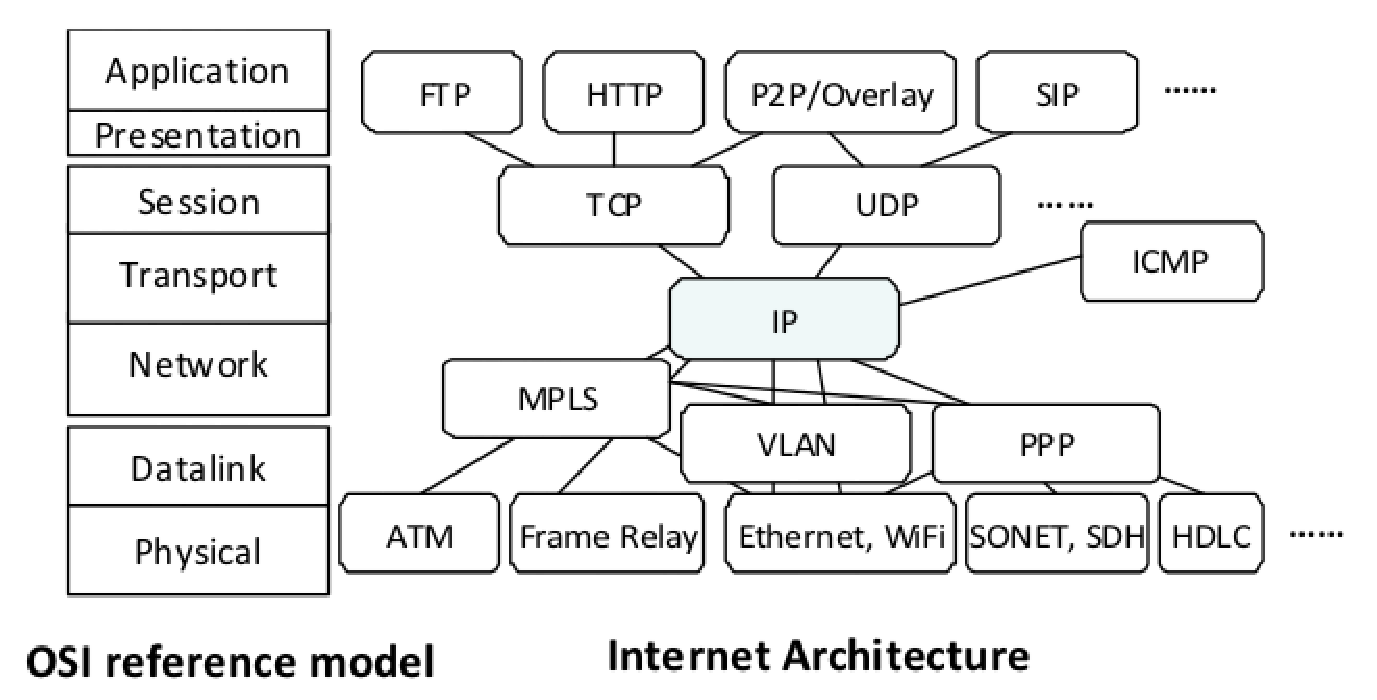
\includegraphics[width=0.7\textwidth]{Figures/protostack-crop.pdf} %	** if .eps or .pdf, don't need extension}
\caption{OSI reference model and IP networking architecture \cite{miya}.}
\label{f:conv}
\end{figure}
%
The development of wireless technology entails however substantial changes in the way that networks are usually represented and conceived. Characteristics of spontaneous wireless networks cannot be handled exclusively at lower layers of communication, as they challenge some of the key assumptions of the IP-based networking architecture. They need thus to be taken into account at layer 3. As more flexible wireless networks are deployed and get increasingly interconnected and integrated with other networks --or in the Internet--, the use of IP over these networks need thus to be adapted or reconsidered. The {\bf first contribution} of the chapter is a review of these considerations, as it elaborates on how the IP-based network architecture is challenged by spontaneous wireless networks.
%
\subsection{Mobile Ad hoc and Low-Power Lossy Networks}
\label{ss:manet_lln}
%
IP protocols are developed, standardized and maintained by the Internet Engineering Task Force (IETF \cite{IETF}). Most of the IETF's protocol design and standardization activities have so far focused on two categories of spontaneous wireless networks: Mobile Ad hoc Networks (MANETs) and Low-Power Lossy Networks (LLNs).

% ({\em e.g.}, a \glslink{router}{router} with multiple \glslink{host}{hosts} and wireless communications devices)--herein simply referred to as `nodes'--

\paragraph{Mobile Ad hoc Networks (MANETs)} According to the IETF's terminology (defined in RFC 2501 \cite{rfc2501}), a MANET consists in a set of ``mobile platforms (..) --herein simply referred to as `nodes'-- (..) which are free to move about arbitrarily. The nodes may be located in or on airplanes, ships, trucks, cars, perhaps even on people or very small devices, and there may be multiple \glslink{host}{hosts} per \glslink{router}{router}. A MANET is an autonomous system of mobile nodes. The system may operate in isolation, or may have gateways to and interface with a fixed network" \cite{rfc2501}. Note that this definition {\em allows} \glslink{router}{router} mobility, but it is {\em not restricted} to mobile networks; the term includes all wireless multi-hop ad hoc networks, regardless of whether they are static or not. 

\paragraph{Low-Power Lossy Networks (LLNs)} According to the IETF's terminology (defined in {\tt draft-ietf-roll-terminology-12}\footnote{An Internet-Draft in the Last Call for becoming an RFC, at the the time of writing this chapter.} \cite{draft_lln}), LLNs are ``typically composed of many embedded devices with limited power, memory, and processing resources interconnected by a variety of links, such as IEEE 802.15.4, LowPower WiFi" \cite{draft_lln}. LLNs are thus a more specific case of MANETs (as defined in the previous paragraph), in which \glslink{router}{routers} typically operate with constraints on processing power, memory, and energy (battery power). Their interconnections are characterized by high loss rates, low data rates, and link instability.  LLNs are comprised of anything from a few dozen to thousands of \glslink{router}{routers}.  Supported traffic flows include point-to-point (between devices inside the LLN), point-to-multipoint (from a central control point to a subset of devices inside the LLN), and multipoint-to-point (from devices inside the LLN towards a central control point). Alternative, but similar terminology is employed in {\tt draft-ietf-lwig-terminology} \cite{bormann13}, which defines the terms ``constrained nodes" and ``constrained networks" with various classes of constraints. \\

Concrete examples of MANETs and LLNs include the following three use cases, selected only for illustrative purposes, to hint at the wide heterogeneity of features, requirements and user expectations that one must address in spontaneous wireless networking.

\paragraph{Vehicular Ad hoc Networks (VANETs)} Communication in VANETs is enabled between moving vehicles in urban scenarios or roadways, (possibly) with fixed devices installed in Roadside Units (RSUs) along the road/street. The combination of vehicles and RSUs forms a mobile, highly dynamic ad hoc network. Devices participating in vehicular networks (either inside vehicles or in RSUs) have neither significant energy constraints nor severe computational limitations, but those installed in vehicles are not, in general, cooperative and willing to dedicate resources to others' communication. Research in these networks has typically focused on safety applications, such as distribution along the highway of information about traffic-related events -- \emph{e.g.}, jams or accidents \cite{bc_vanet}. Other purposes could be also considered, such as dissemination of service availability along the highway (gas stations, tolls, accommodation, etc.). As such, a VANET is a category of MANET.

\paragraph{Community Wireless Mesh Networks} These are cooperative, non-commercial networking projects in which users join and contribute to the deployment of the network, in particular by sharing resources and allowing the use of their devices as networking relays. Several initiatives have flourished in the last years, such as Spain's {\em Guifi} \cite{GUIFI}, mostly deployed over the Eastern coast of Spain (Catalonia and Valencia) but also present in many other parts of the country. Other examples include Germany's {\em Freifunk} \cite{FREIFUNK} and Austria's {\em Funkfeuer} \cite{FUNKFEUER}. Some of them cover large geographical areas and contain thousands of nodes\footnote{{\em Guifi.net}, for instance, claims 31865 nodes, 20425 of them being ``operating nodes" (last query to {\tt http://www.guifi.net} on April 10th, 2013).}. These networks are typically static, most of the links are wireless links operating in free (unlicensed) frequency bands. Their topology and capacity evolve dynamically, in an unplanned manner, subject to events such as the ingress and egress of users, the subsequent availability of new links and resources or the upgrade of a particular networking region. These networks enable free communication among their users, but they can also provide access to the Internet if there are gateways available. As such, a community wireless mesh networks is also a category of MANET.

\paragraph{Wireless Sensor Networks (WSNs)} WSNs are collections of sensors intended to measure one or several properties of the environment in which they are deployed. Communication facilities required by such networks need to include, at least, the transmission of collected information from the sensors to a gateway or central server that stores and eventually process it, and the transmission of information (\emph{e.g.}, configuration instructions or measurement schedules) from the server to one or more sensors. There is a broad range of information that may be collected and exchanged through WSNs, some examples including climate studies, bird observation, power monitoring in buildings or tracking of patients' health parameters with body sensors. Properties of a WSN may vary depending on the purposes of the sensor deployment, but there are some usual constraints. Sensors are often battery driven, the lifetime of the sensor is limited by the battery lifetime. Protocols for enabling communication within WSNs must therefore be designed with energy consumption and energy-efficiency in mind. As such, a wireless sensor network is a category of LLN.\\

Despite their heterogeneity, these use cases -- and other applications of spontaneous wireless networks -- have common characteristics, including bandwidth scarcity and need for self-organization. These characteristics both require the use of efficient, highly decentralized routing and flooding mechanisms, able to react quickly to topology changes without overloading the network. This chapter thus focuses more specifically  on IP protocols that enable routing and flooding in MANETs and LLNs. While plenty of protocols have been proposed in the literature, only few have been effectively implemented, standardized and used in real-world deployments. The {\bf second contribution} of the chapter consists in:

\begin{enumerate}[(1)] 
\item an analysis of the main implications of wireless mesh characteristics on the task of flooding and routing typically implemented in upper-layer protocols; and 
\item a description and discussion of the key mechanisms and operation of the main protocols deployed so far and standardized at the IETF for routing in MANETs, in LLNs and in heterogeneous wired/wireless inter-networks.
\end{enumerate}

\subsection{Reader's Guide}

Reader is assumed to be familiar with the main concepts of computer networking and the TCP/IP network reference model, whose terminology is used in this chapter. Interested readers are referred to the book of Tanenbaum {\em et al.} \cite{tanenbaum} for details; the glossary at the end of the chapter displays standard definitions of the basic networking concepts. Basic knowledge of the Internet Protocol (IP) operation, addressing model, routing and Internet architecture is also preferable, but not necessary. These elements are briefly overviewed in section \ref{s:fundamentals}, in order to better highlight the issues that arise with the traditional IP model in spontaneous wireless networks, addressed in section \ref{s:comm_wless}. This section describes the conditions under which wireless communication occurs, and examines their impact on the communication performance and the architecture of spontaneous wireless networks. In particular, the section explains the non-suitability of the conventional IP networking model for spontaneous wireless networks, and discusses an alternative model. \ \\ \ \\ 
%
The rest of the chapter focuses on the mechanisms and protocols that have been designed to handle flooding and routing in spontaneous wireless networks, paying a particular attention to the efforts deployed at the IETF. Section \ref{s:flood_rtg} motivates and presents the mechanisms, and section \ref{s:specific} describes the routing and flooding protocols that have been specifically designed in the IETF to operate on MANETs and LLNs. Section \ref{s:wospf} focuses on the problem of extending legacy Internet routing protocols so that they can efficiently operate on hybrid (wired/wireless) inter-networks. Finally, section \ref{sec:conclusion} concludes the chapter.

\section{Fundamentals of IP Networking and Internet Routing}
\label{s:fundamentals}

This section introduces the main ideas and concepts that are used as a basis for traditional wired Internet. Subection \ref{ss:ip} presents the key elements of the IP networking model, including addressing, forwarding and the notion of IP link. Subection \ref{ss:routing} describes the most relevant routing techniques used in the Internet, and subsection \ref{ss:irarq} overviews the Internet routing architecture, based on the notion of Autonomous System. A certain familiarity with the basics of computer networking is assumed, so no details are provided. This section mainly follows the classic manuals of Tanenbaum {\em et al.} \cite{tanenbaum}, Comer \cite{comer} and Perlman \cite{interconnections}. Interested readers are referred to these resources for further explanations. \ \\ \ \\
% Assumptions:
% - TCP/IP stack
%
%This chapter focuses on communication in layer 3 (internetworking) for multi-hop IP networks (partly) composed of wireless links. Protocols and devices operating at this layer enable communication between hosts not belonging to the same link. 
%
\subsection{The IP Networking Model}
\label{ss:ip}
%
The Internet Protocol (IP) defines the key elements enabling communication in an IP network. This section presents the IP addressing mechanism, the notion of IP link and the routing rule used by router in IP networks -- the {\em longest prefix match} criterion.
%
\paragraph{Addressing}

In an IP network, every \glslink{interface}{\em network interface} is assigned at least one {\bf IP address} that identifies unambiguously the \glslink{interface}{interface} in the network. The IP address format varies depending on the protocol version (32 bits for IPv4, 128 bits for IPv6, see Figure \ref{f:ipa}), but three elements  can be distinguished.

\begin{itemize}
\item The {\bf host identifier} is the set of bits that identifies the \glslink{interface}{interface} in the network.
\item The {\bf network prefix} is the set of bits that identifies the network to which the \glslink{interface}{interface} is attached.
\item The {\bf network mask} allows to obtain the network prefix and the host identifier from the IP address. 
\end{itemize}

\begin{remark}
The IP address of a network \glslink{interface}{interface} is both an {\em identifier} and a {\em locator} of the interface: it indicates {\em who} is (unambiguosly in the internetwork) the attached \glslink{interface}{interface} and {\em where} is it attached (to which network).
\end{remark}

\begin{figure}[htb]
\centering
{\small a) IPv4 addressing example: $192.168.0.1/24$}
\begin{eqnarray*}
\textrm{Mask (24):} 		& \underbrace{{\tt 11111111}.{\tt 11111111}.{\tt 11111111}}_{\textrm{netmask (24 bits)}}.{\tt 00000000} \\
\textrm{IP address:} 	& \underbrace{{\tt 11000000}.{\tt 10101000}.{\tt 00000000}}_{\textrm{network prefix}}.\underbrace{{\tt 00000001}}_{\textrm{host identifier}}
\end{eqnarray*}
{\small b) IPv6 addressing example: $2001:0DB8:02DE::0E13/64$}
\begin{eqnarray*}
\textrm{Mask (64):} 			& \underbrace{{\tt FFFF}:{\tt FFFF}:{\tt FFFF}:{\tt FFFF}}_{\textrm{netmask (64 bits)}}:{\tt 0000}:{\tt 0000}:{\tt 0000}:{\tt 0E13} \\
\textrm{IP address:} 	& \underbrace{{\tt 2001}:{\tt 0DB8}:{\tt 02DE}:{\tt 0000}}_{\textrm{network prefix}}:\underbrace{{\tt 0000}:{\tt 0000}:{\tt 0000}:{\tt 0E13}}_{\textrm{host identifier}}
\end{eqnarray*}
\caption{IP address structure, for IPv4 and IPv6.}
\label{f:ipa}
\end{figure}
%
%\begin{remark}
%In the context of an IP network, a routing table is a local database that maps IP prefixes (from packet destinations) to the networking \glslink{interface}{interface} and the IP address of the next hop (to which the packet should be sent).
%\end{remark}
%
Based on the information contained in IP addresses from the destination field of the IP header, routers and hosts are able to take decisions upon reception of an IP packet. Trivially, a host receiving an IP packet will accept it only in case that the destination IP address is itself\footnote{Or the destination address is a broadcast address or a multicast address to which the host has suscribed.} and drop it otherwise. A router receiving an IP packet over an \glslink{interface}{interface} will compare the network prefix of the destination IP address with the prefix of its own interface: if it does not match, it may forward it through another interface, according to the IP forwarding rule (see below). In case of forwarding, the router decreases the {\em Time-To-Live} field (or {\em hop-limit} for IPv6), to indicate that the corresponding packet has traversed one (more) router in its path to its destination. This leads to the notion of \glslink{ip-link}{\em IP link} (see Figure \ref{f:iplink}).
%
\begin{definition}[IP Link]
Two network interfaces, $x$ and $y$, are connected to the same {\em IP link} when they can exchange packets in an IP network without requiring that any router forwards them, that is, when packets sent from one \glslink{interface}{interface} are received in the other with the same TTL/hop-limit value. This relationship is denoted as $x \sim_{IP} y$.
\end{definition}
%
\begin{itemize}
\item In these conditions, communication is performed in a single {\em IP hop}.
\end{itemize}

%Let $\sim_{IP}$ denote the IP link relationship, by which $x \sim_{IP} y$ if and only if network interfaces $x$ and $y$ belong to the same IP link, and let $a$, $b$ and $c$ be network interfaces. Definition~(\ref{d:ip_link}) implies the following properties of IP links:

\begin{remark}
Let $a$, $b$ and $c$ be network interfaces. The previous definition implies the following properties of IP links:

\begin{itemize}
\item \emph{Symmetry}: $a \sim_{IP} b \Longleftrightarrow b \sim_{IP} a$.
\item \emph{Transitivity}: $a \sim_{IP} b, b \sim_{IP} c \Longrightarrow a \sim_{IP} c$.
\end{itemize}
\end{remark}

Note that transitivity does {\em not} hold in terms of routers. The fact that a router $R_1$ and a router $R_2$ are connected to the same link, and $R_2$ and $R_3$ are connected to the same link, does not imply that $R_1$ and $R_2$ have a link in common: $R_2$ may be attached to two different links (one connecting with $R_1$ and another with $R_3$) by way of two different network interfaces.

\begin{figure}[htb]	% H-must be here or [htb]
\centering
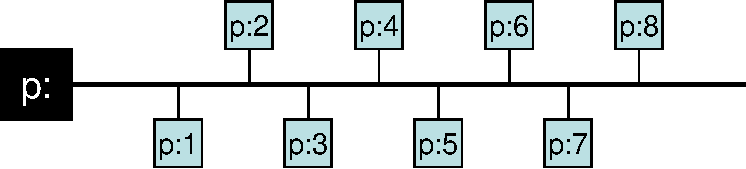
\includegraphics[width=0.5\textwidth]{Figures/iplink-crop.pdf} %	** if .eps or .pdf, don't need extension}
\caption{An IP link {\tt p:} with network prefix $p$. \emph{IP addresses of nodes in this IP link have the structure {\tt p:i}$/[p]$, for $0 < i < 2^{[p]}$.}}
\label{f:iplink}
\end{figure}

\paragraph{Forwarding rule}

When source and destination of a packet do not belong to the same IP link, routers receiving the packet compare the IP address of the destination to the prefixes stored in the routing table, and forward the packet through the network \glslink{interface}{interface} corresponding to the prefix showing the {\em longest prefix match}, this is, the prefix in the routing table for which a bigger number of bits are coincident with those from the network prefix of the IP address of the packet destination. %This is the {\em closest} prefix towards the destination, according to the IP closeness notion and the IP ordering criterion over the addressing space induced by the definition of IP link.

%\begin{definition}[IP Partial Order]
%Given two IP addresses $IPA_1/m_1$ and $IPA_2/m_2$ ($m_i$ being the prefix length of IP address $IPA_i$), $IPA_1 \subseteq_{IP} IPA_2$ if and only if:
%\begin{enumerate}[(i)]
%\item $IPA_1 \otimes NM_{\textrm{ max}\{m_1, m_2\}} = IPA_2 \otimes NM_{\textrm{ max}\{m_1, m_2\}}$ 
%\item $m_1 \geq m_2$
%\end{enumerate}
%where $NM_k$ is the netmask of $k$ bits and $\otimes$ denotes the bitwise AND operation.
%\end{definition}

%\begin{remark}
%The relationship $\subseteq_{IP}$ satisfies trivially the axioms of partial order:
%	\begin{itemize}
%	\item \emph{Reflexivity}: $IP_a \subseteq_{IP} IP_a$.
%	\item \emph{Antisymmetry}: $IP_a \subseteq_{IP} IP_b, IP_b \subseteq_{IP} IP_a \Longrightarrow IP_a \sim_{IP} IP_b$, that is, $IP_a$ and $IP_b$ are in the same IP link.
%	\item \emph{Transitivity}: $IP_a \subseteq_{IP} IP_b, IP_b \subseteq_{IP} IP_c \Longrightarrow IP_a \subseteq_{IP} IP_c$.
%	\end{itemize}
%\end{remark}

%For routing of packets for which the IP link of the destination is not the same as the IP link of the source, the IP addressing model provides a simple rule for making forwarding decisions. Given the IP address of the packet’s destination, a router should forward the packet through the \glslink{interface}{interface} providing connection to the IP network closest to the destination, where the notion of {\em closeness} is as follows:

%\begin{definition}[IP Closeness]
%Given an IP address $IPA_d/m_d$ and two IP addresses $IPA_1/m_1$ and $IPA_2/m_2$, $IPA_1/m_1$ is \emph{IP-closer} to $IPA_d/m_d$ than to $IPA_2/m_2$ if:
%	\begin{itemize}
%	\item $IPA_d \subseteq_{IP} IPA_1$ and $IPA_d \not\subseteq_{IP} IPA_2$, or
%	\item $IPA_d \subseteq_{IP} IPA_1 \subseteq_{IP} IPA_2$ (which is equivalent to $|m_1| \geq |m_2|$, for the case $IPA_d \subseteq_{IP} IPA_{1,2}$).
%	\end{itemize}
%\end{definition}

%According to this decision criterion, routers select send a given IP packet to the \glslink{interface}{interface} whose IP address has the \emph{longest prefix match} with respect to the IP packet destination. 

%\begin{remark}
%Note that the longest prefix match is only guaranteed to exist if and only if the router has a \emph{default route} ({\tt 0.0.0.0/0} in IPv4, {\tt ::/0} in IPv6).
%\end{remark}

\subsection{Main Routing Techniques}
\label{ss:routing}
%
Two types of routing techniques currently dominate \cite{interconnections}: {\em link-state} routing and {\em distance-vector} routing (with the variant of {\em path-vector} routing). The main protocols used historically and currently in the Internet are based on these techniques.
%
\paragraph{Link-State Routing} Routers advertise the status of their links (link-state) to the whole network. Link status may include information about the type of link (broadcast, point-to-point...), the link communication capabilities (one-directional, bi-directional, link cost) or the routers to which communication is available through this link. This way, every router in the network receives the link-state of other routers in the network, maintains information about the whole network topology and is therefore able to locally compute network-wide shortest paths, usually by way of Dijkstra's algorithm \cite{dijkstra59}. 
	\begin{itemize}
	\item Some examples of this approach are the Open Shortest Path First (OSPF, RFCs 2328 and 5340 \cite{rfc2328,rfc5340}) and the Intermediate System to Intermediate System (IS-IS, RFC 1142 \cite{rfc1142}) protocols, as well as the Optimized Link State Routing protocol (OLSR, RFC 3626 \cite{rfc3626}).
	\end{itemize}

\paragraph{Distance-Vector Routing} A router shares information from its routing table only with its neighbors, indicating \emph{distances} and next hops towards reachable destinations. Neighbor distance is defined according to the current \glslink{metric}{\em link metric}, which maps links between routers with estimations of the cost of sending packets through them, represented by scalar values. By receiving the routing tables of all its neighbors, which in turn have been shared with the neighbors of the neighbors, a router is able to identify, for each advertised destination, the neighbor that provides shortest distance and select it as next hop. Distance-vector protocols mostly use the distributed Bellman-Ford algorithm \cite{bellman58,ford56} to identify network-wide shortest paths. 
	\begin{itemize}
	\item The Routing Information Protocol (RIP, RFCs 1058 \cite{rfc1058}, 2080 \cite{rfc2080} and 2453 \cite{rfc2453}) is a prominent example of this family.
	\end{itemize}

\paragraph{Path-vector routing} It is based on the same principle as distance-vector routing, a router advertises to its neighbors the paths to all reachable destinations. Each path is described by indicating the routers that are traversed. This way, local distribution of locally maintained paths enables all routers in the network to build routes to all possible destinations. 
	\begin{itemize}
	\item The most prominent example of this family of protocols is the Border Gateway Protocol (BGP, RFC 1771 \cite{rfc1771}). \\
	\end{itemize}

% -------------
The link-state algorithm requires that every single router has storage and computational capacity to compute locally the shortest-path tree of the network, based on the information received from every other routers, and extract from that tree the next-hop towards every destination in the network. Distance-vector algorithms only require that each router updates the distance-vectors received from their neighbor to infer its own vector of distance vector and select its next-hops. \ \\ \ \\
%
Due to their computational simplicity, distance-vector protocols were used in the early stages of the Internet. They were gradually replaced by link-state protocols as the ARPANET grew bigger and more complex, due to problems such as the well-known count-to-infinity problem \cite{tanenbaum} (which appears in the original distance-vector algorithm, but does not appear on path-vector protocols). Poor scalability and slow convergence properties of distance-vector with respect to link-state algorithms were also major reasons to switch from one technique to the other \cite{interconnections}.

\begin{itemize}
\item The network reaction to a link failure illustrates the differences between link-state and distance-vector algorithms in terms of convergence. In distance-vector algorithms, once a router detects such a failure, it updates the cost of its route towards the lost neighbor and sends the new vector of distances to its neighbors. Neighbors receive this update and {\em recompute} the cost of the affected route, and then transmit in turn their new vectors. Propagation of topology changes is thus slower than in link-state algorithms, in which a router detecting the failure of the link towards one of its neighbors {\em floods} an updated topology description which is directly forwarded over the network, without delays caused by route re-computation in intermediate routers \cite{interconnections}.
\end{itemize}
% ------------------

Routing protocols for wired networks used to be {\em proactive} or table-driven, in which next hop to any possible destination is stored in a table.  With the emergence of wireless networks and, more generally, more dynamic networking architectures coping with more scarce (shared) bandwith, {\em reactive} routing protocols were then designed and deployed, in which routes were only computed upon request (on-demand).

\paragraph{Proactive routing} Routers collect and periodically disseminate topology information over the network; this enables them to maintain proactively (\emph{i.e.}, regardless on whether they are used) routes towards all destinations. This way, routers are able to forward packets at any time to any destination in the network.

\paragraph{Reactive routing} A router calculates a route to a destination only when it receives packets addressed to that destination and the routing table does not provide a next hop towards it. In this case, the router triggers a {\em route discovery} process by disseminating a Route Request (RREQ) packet through the network. The route discovery process terminates when the requested destination or another router knowing a valid route towards the destination reply to the requesting router.  
	\begin{itemize}
	\item Dynamic Source Routing (DSR, RFC 4728 \cite{rfc4728}) or Ad hoc On-Demand Distance Vector (AODV, RFC 3561 \cite{rfc3561}), both used in spontaneous wireless networks, are examples of reactive routing protocols. \\
	\end{itemize}

Proactive maintenance of next hops to every possible destination in the table requires a constant exchange of control traffic in the network, but enables routers to forward packets immediately after receiving them. Reactive protocols adapt the control traffic to the data traffic requirements: when there is no traffic to route, or the traffic follows known paths, a mostly negligible amount of control traffic (very low or even zero, depending on the protocol) is needed. When a router receives packets to be sent to a destination for which no route is known, the router needs to address a route discovery process over the network -- such a discovery process is costly in terms of overhead, and leads to significant delays in the forwarding.

\paragraph{Other routing approaches} Some other approaches have been explored for routing over spontaneous wireless networks. In some cases, they rely on additional assumptions about properties and capabilities of the involved devices. If nodes' position is available (for instance, by way of GPS), {\bf geographical routing} approaches are possible: in these protocols, a packet is forwarded to the relay getting closer to the final destination. The Greedy Perimeter Stateless Routing (GPSR) protocol \cite{gpsr} was the first protocol exploring this principle.

%\begin{tabular}{|c||c|c|}
%\hline
%    		& Proactive 		& Reactive  	\\ \hline\hline
%Link-State 	& OSPF, IS-IS, OLSR 	& 		\\ \hline
%Distance-Vector	& RPL, RIP, BGP 	& AODV, LOAD	\\ \hline
%\end{tabular}


%\subsubsection{Other Approaches}

%\begin{itemize}
%\item Opportunistic routing. ExOR.
%\item Source routing. DSR.
%\end{itemize}

\subsection{The Internet Routing Architecture}
\label{ss:irarq}

In terms of routing, the Internet is organized as a set of interconnected internetworks, denominated {\em Autonomous Systems} (see Figure \ref{f:ass}). The networks in each Autonomous System are under the same administrative control, and are assumed to perform routing inside the AS {\em autonomously} from the rest of networks in the Internet. The formal definition of an AS is as follows:

\begin{definition}[Autonomous System]
``An \emph{Autonomous System (AS)} is a connected group of one or more IP prefixes [internetwork] run by one or more network operators which has a SINGLE and CLEARLY DEFINED routing policy" \cite{rfc1930}, the term ``routing policy" denoting the way that routing information is exchanged between (but not within) Autonomous Systems. In the interior of an AS, ``routers may use one or more interior routing protocols, and sometimes several sets of \glslink{metric}{metrics}" \cite{rfc1812}.
\end{definition}

\begin{figure}[htb]	% H-must be here or [htb]
\centering
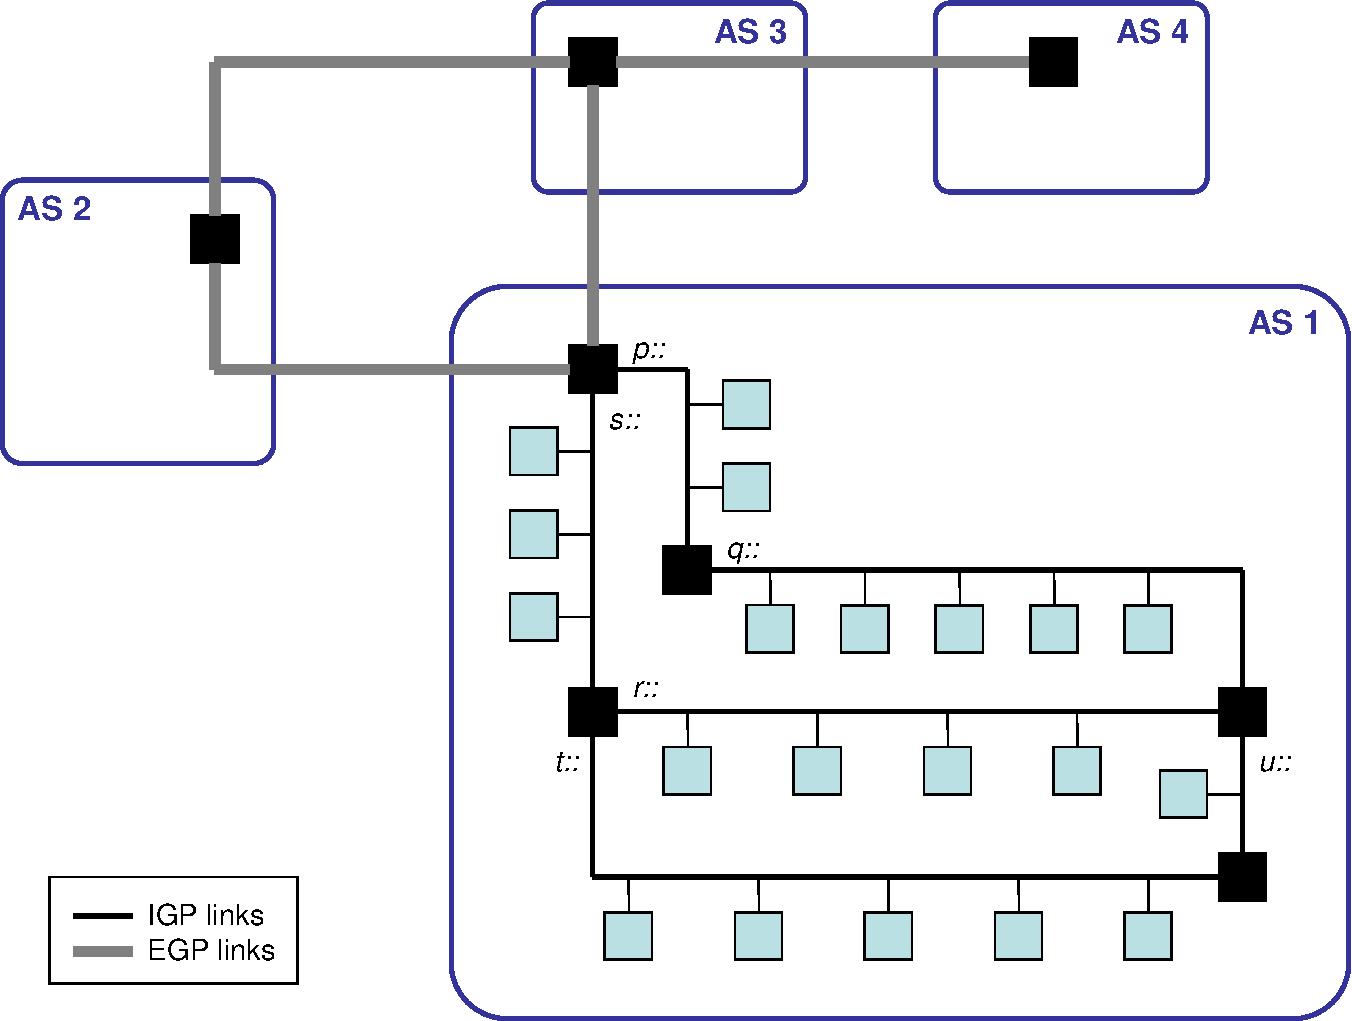
\includegraphics[width=0.8\textwidth]{Figures/ass-crop.pdf} %	** if .eps or .pdf, don't need extension}
\caption{Connection of different Autonomous Systems.}
\label{f:ass}
\end{figure}

The distinction between routing inside an Autonomous System (intra-AS or intra-domain routing) and routing between different ASes (inter-AS or inter-domain routing) leads to two different types of routing protocols: 

\begin{enumerate}[(i)]
\item {\em Interior Gateway Protocols} (IGPs), for route discovery and maintenance within an Autonomous System. Intra-domain routing is mostly performed by way of link-state protocols; the most significant link-state routing protocol for TCP/IP networks in the Internet are the Open Shortest Path First protocol (OSPF, \cite{rfc2328, rfc5340}, described in section \ref{s:wospf}) and the Integrated IS-IS, an IP variant of the Intermediate Systems to Intermediate Systems (IS-IS) protocol (see \cite{rfc1195}).
\item {\em Exterior Gateway Protocols} (EGPs), for route acquisition and information exchange between different Autonomous Systems. The current standard protocol for inter-domain routing is the path-vector Border Gateway Protocol (BGP, \cite{rfc1771}).
\end{enumerate}



\section{Communication in Spontaneous Wireless Networks}
\label{s:comm_wless}

This section describes the basics of communication between wireless devices and presents the main implications for spontaneous wireless networks at layer 3. Physical limitations and derived properties are examined in section \ref{s:phy}. The implications of these properties in the networking model for spontaneous wireless networks, and in particular the suitability of the IP model, are detailed in section \ref{ss:ip}, is discussed in section \ref{ss:issues}. Finally, section \ref{ss:model} describes an IP-compatible networking model for multi hop communication in spontaneous wireless networks.

\subsection{Physical Aspects of Wireless Communication}
\label{s:phy}

The fact that two wireless devices in a wireless network are able to communicate to each other depends of several factors (see Figure \ref{f:wlessab}), and some of them are not related to any of the involved devices. The most significant factors include:

\begin{enumerate}[(i)]
\item The distance between two devices.
\item The physical properties of the transmitting and receiving antennas: number of transmission/reception antennas, transmission power and antenna directivities.
\item Network dynamics: in mobile networks, depending on the relative motion of wireless devices involved in communication, the Doppler frequency shift may have a non-negligible impact.
\end{enumerate}

The modulation and coding schemes used to transmit and receive packets have impact in other physical factors of the transmission, including:

%\item The physical properties of the transmitting and receiving antennas and of the transmission itself: modulation scheme, transmission power, antenna directivities.

\begin{enumerate}[(i)]
	\setcounter{enumi}{3}
\item The characteristics of the wireless medium: signal frequency band, noise power, effect of weather conditions or {\em interferences} from other devices transmitting in close frequency bands.
\item The physical topology of the {\em coverage} area: fading caused by obstacles, reflection and absorption causing multi-path interference and signal loss.
%The state of the electromagnetic spectrum in the environment: weather conditions or interferences from other transmitters. 
\end{enumerate}

\begin{figure}
\centering
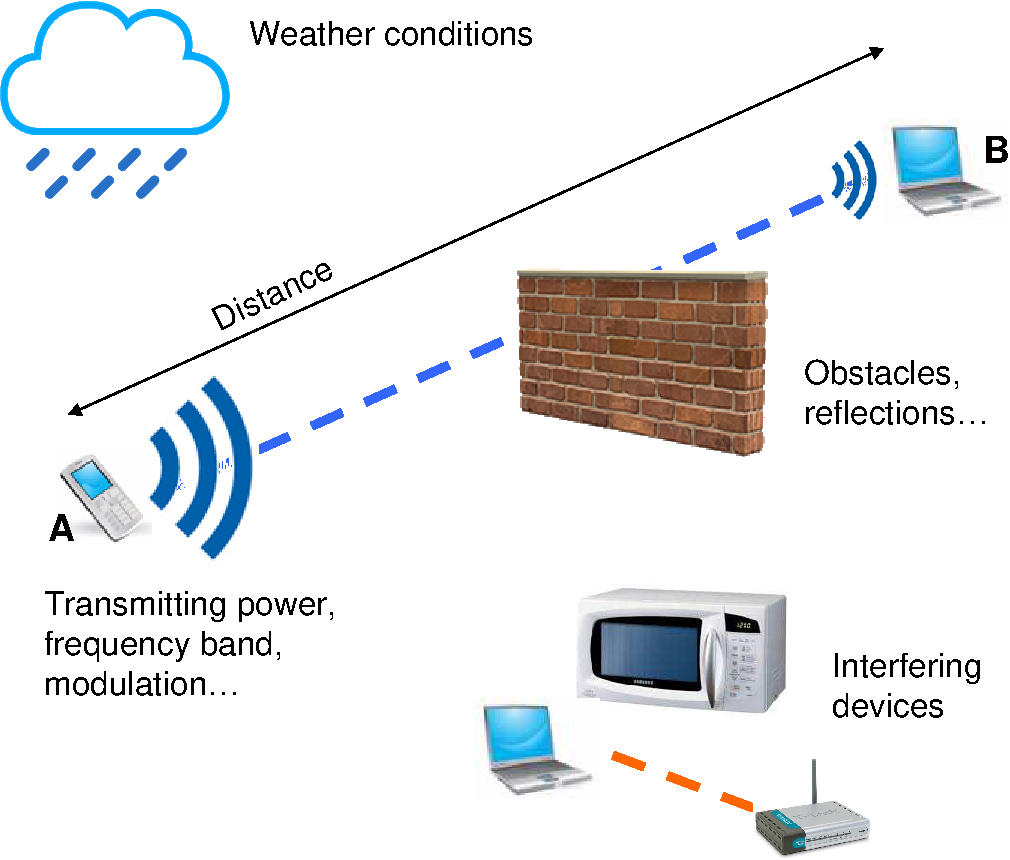
\includegraphics[width=0.60\textwidth]{Figures/wirelessab-crop.pdf}
\caption{Communication between wireless devices $A$ and $B$}
\label{f:wlessab}
\end{figure}

Note that, as some of these factors are time-variant and their impact may change rapidly, {\em e.g.} (iv), some links (or all of them) may have intermittent availability, even if devices keep static.

\paragraph{Coverage and Interference}

The concepts of {\em coverage} and {\em interference} have been mentioned in the previous list, and are some of the key parameters that define the behavior and impact of a wireless interface in a spontaneous wireless network.

\begin{definition}[Coverage Area]
Given a wireless interface $A$, the \emph{coverage area} of $A$ is the geographical region in which packets transmitted by $A$ can be received and correctly decoded by other interfaces on the same wireless medium as $A$, when no competing transmission is ongoing. The coverage area of $A$ is denoted by $Cov(A)$.
\end{definition}

\begin{definition}[Interference Area]
Given a wireless interface $A$, the \emph{interference area} of $A$ is the geographical region in which interfaces connected to the same wireless medium as $A$ may be unable to receive or correctly decode other packets when there is an ongoing transmission from $A$. The interference area of $A$ is denoted by $Intf(A)$.
\end{definition}

\begin{remark}
Note that, the coverage area of a wireless networking interface is always contained in the interference area of that interface, that is, $Cov(A) \subseteq Intf(A) \forall A$, as shown in the following and represented in Figure \ref{f:cov_intf}.
	\begin{itemize}
	\item Let $T>1$ be the SINR (Signal-and-Interferece-Noise-Ratio) threshold for receiving and decoding correctly packets from a wireless interface. That means that a transmission ({\em e.g.}, from $A$) is received and correctly decoded by the receiver, in absence of competing transmissions, if $\textrm{SINR}|_{I=0}=\textrm{SNR}=\frac{S}{N} > T$ and discarded otherwise. As received power decreases quadratically with distance from the transmitter, let $S(d)=\frac{P}{d^2}$. Then, the maximum coverage distance is $d_c=\sqrt{\frac{P}{NT}}$. The maximum distance at which there may be interference (from $A$), $d_i$, corresponds to the distance to a receiver $B$ such that another transmitter, $C$, transmitting with the same power $P$ at any distance $d\leq d_c$ from $B$, would be unable to send successfully a packet in case of concurrent transmission from $A$. This is, $T=\textrm{SINR}|_{N \ll I}=\textrm{SIR}=\frac{P/d_{BC}^2}{P/d_i^2}$. In the worst case, $d_{BC} = d_c$ and $\frac{P/d_{BC}^2}{P/d_i^2} = \frac{d_{i}^2}{d_c^2} = T$, and therefore $d_i<d_c$.
	\end{itemize}
\end{remark}

% added -------------------------------
\begin{comment}

\emph{Proposition \ref{p:cov_intf}} defines the coverage and interference areas under the conditions of the Friis' Transmission Equation (\ref{e:free}), and shows in particular that the latter is bigger than the former.

{\small
	\begin{theorem}
	\label{p:cov_intf}
	Let $a$ be a wireless interface in a wireless network, in which information propagates under free space conditions. Let $P$ be the power at which all interfaces transmit in the network, and $N$ the noise power, assuming an AWGN\footnote{Additive White Gaussian Noise.} model. Let $T>1$ be the minimum signal-to-interference-and-noise ratio (SINR) for a transmission to be successfully decoded by $a$. 
	Then, the coverage area of $a$ is a circle centered in $a$ with radius $r=4\pi \sqrt{\frac{P}{NT}}$, and the interference area of $a$ is a circle centered in $a$ with radius $r_i=4\pi\sqrt{\frac{P}{N}}$. As $T>1$, $r_i>r$.
	\end{theorem}
	\begin{proof} The coverage area of $a$ is the geographical region in which the SINR of the received signal is higher than $T$, in absence of other transmissions (def.~ \ref{d:cov}). If not other transmissions occur, there is no interference ($I=0$), and the SINR for an interface $b$, at distance $d$ of $a$ becomes the signal-to-noise ratio, SNR of $b$.
		\begin{equation*}
		SINR|_b = \left.\frac{S}{N+I}\right]_b = [I=0] = \left.\frac{S}{N}\right]_b = SNR|_b
		\end{equation*}
	Applying the Friis Transmission Equation (\ref{e:free}) and assuming unitary gains $G_r,G_t=1$,
		\begin{eqnarray*}
		SNR|_b = \left.\frac{S}{N}\right]_b > T \\
		\frac{P\left(\frac{\lambda}{4\pi d}\right)^2}{N} > T \\
		d < 4\pi \sqrt{\frac{P}{NT}} = r
		\end{eqnarray*}
	When $d<r$, an interface at distance $d$ from $a$ is able to receive packets transmitted from $a$.
	For the interference area (def.~ \ref{d:intf}), consider the case when an interface $b$ at distance $d$ receives signals from $a$ and from another (neighboring) interface, $c$, at distance $d_o$ from $b$. Transmission from $a$ causes interference with a transmission from $c$, in $b$, if the SINR at $b$ is lower than $T$. Considering that the impact of the noise is negligible with respect to interference ($N \ll I$):
		\begin{eqnarray*}
		SINR_b \approx SIR_b = \left.\frac{S}{I}\right]_b > T \\
		\frac{P\left(\frac{\lambda}{4\pi d}\right)^2}{P\left(\frac{\lambda}{4\pi d_o}\right)^2} > T \\
		d < d_o\sqrt{T}
		\end{eqnarray*}
	Consider the worst case: distance between $b$ and the main transmitter $c$ is maximum, \emph{i.e.}, $r=4\pi \sqrt{\frac{P}{NT}}$. Then:
		\begin{equation*}
		d < \frac{\lambda}{4\pi}\sqrt{\frac{P}{N}} = r_i
		\end{equation*}
	where $r_i$ is the radius of the interference area of $a$.
	\end{proof}
}

\end{comment}
% end added ---------------------------------------------

\begin{figure}[htb]	% H-must be here or [htb]
\centering
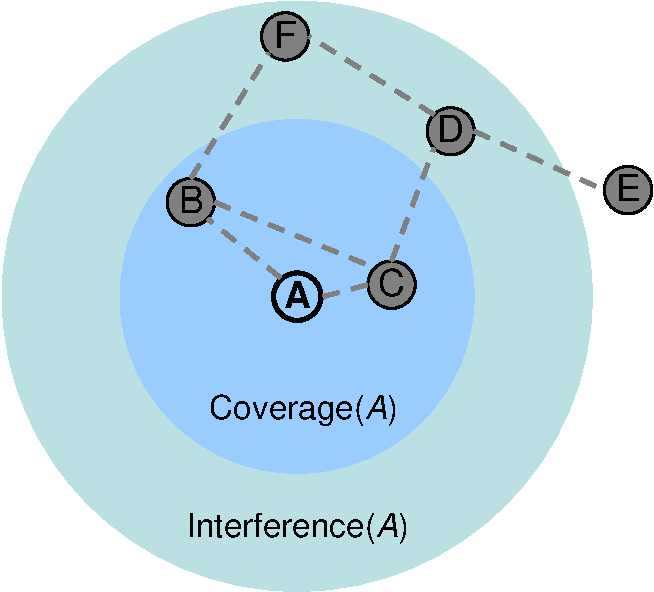
\includegraphics[width=0.40\textwidth]{Figures/cov_intf-crop.pdf}
\caption{Idealized representation of coverage and interference areas of an interface $A$.}
\label{f:cov_intf}
\end{figure}

Due to the variability of factors having impact on wireless communication, coverage and interference areas of an interface are time-variant and in practice their shapes are significantly more irregular than the circles depicted in Figure \ref{f:cov_intf} \cite{kotz03}. Even within the coverage area at a particular time, when communication is possible, a wireless link is inherently unreliable and prone to transmission errors and packet losses \cite{book_wless}, for instance due to interferences from other interfaces in the network or external sources transmitting in the same frequency band. 

\subsection{IP Model Issues in Spontaneous Wireless Networks}
\label{ss:issues}

The properties of wireless medium have severe implications for the characteristics of neighbor relationship at layer 3 (L3) in spontaneous wireless networks. In contrast to the case of wired IP links, neighbor relationships between wireless interfaces are not necessarily {\em symmetric} nor {\em transitive} \cite{baccelli12}. This entails some additional effect that are further illustrated in this section: the {\em hidden node} problem and the {\em exposed node} problem.

\begin{figure}[htb]	% H-must be here or [htb]
\centering
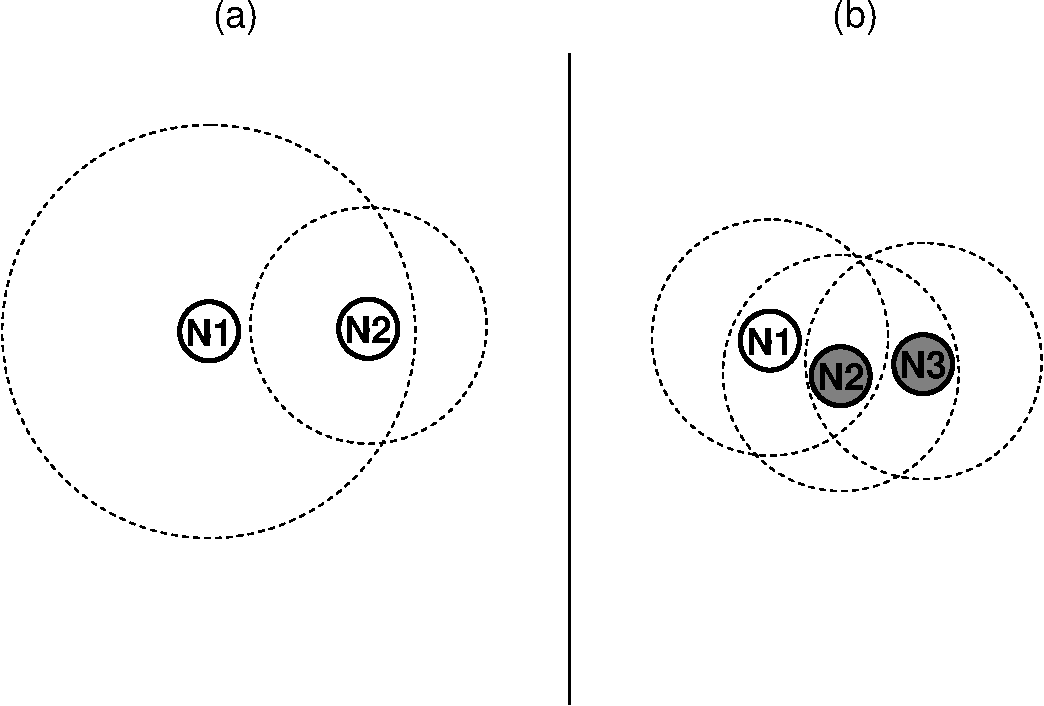
\includegraphics[width=0.7\textwidth]{Figures/asym-crop.pdf} \\
\caption{Asymmetry and non-transitivity in neighbor relationships between wireless interfaces.}
\label{f:asym}
\end{figure}

\paragraph{Non-Symmetric Links}

Consider the small wireless network in Figure \ref{f:asym}.a: for some reason (powerful transmitter, large antenna, ...) the wireless interface of $N1$ has a large enough coverage area that its transmissions can be received by the wireless interface $N2$. The wireless interface of $N2$, on the other hand, has a much smaller coverage radius, such that transmissions from the wireless interface of $N2$ do not arrive at the wireless interface of $N1$. Thus an asymmetric --or more precisely, an unidirectional-- connectivity between the wireless interface of $N1$ and the wireless interface of $N2$ exists: $N2$ sees $N1$ as a neighbor (since the wireless interface $N2$ can receive transmissions from the wireless interface of $N1$), whereas $N1$ does not see $N2$ as a neighbor (since the wireless interface of $N1$ can not receive transmissions from the wireless interface of $N2$). This situation illustrates that neighbor relationships in a wireless network are not necessarily symmetric.

\paragraph{Non-Transitive Links} Figure \ref{f:asym}.b shows a case of non-transitive links in a 2-hop wireless network. $N1$ and $N2$ are neighbors: the wireless interface of $N1$ is inside the coverage area of $N2$, and therefore $N1$'s transmissions are received at the wireless interface of $N2$ -- and viceversa. Observe that the same applies with $N2$ and $N3$: $N2$ and $N3$ are also neighbors. However, direct communication between $N1$ and $N3$ is not possible, as their respective wireless interfaces are outside the coverage area of each other. In a spontaneous wireless network, the fact that $N1$ and $N2$ are neighbors ({\em i.e.}, can communicate directly) and $N2$ and $N3$ are neighbors as well does not imply that $N1$ and $N3$ are neighbors to each other: neighbor relationship in a spontaneous wireless network is not necessarily transitive. \ \\ \ \\
%
These two constraints lead to situations that do not occur in traditional IP networks, such as the {\em hidden node problem} and the {\em exposed node problem}.

\begin{figure}[htb]	% H-must be here or [htb]
\centering
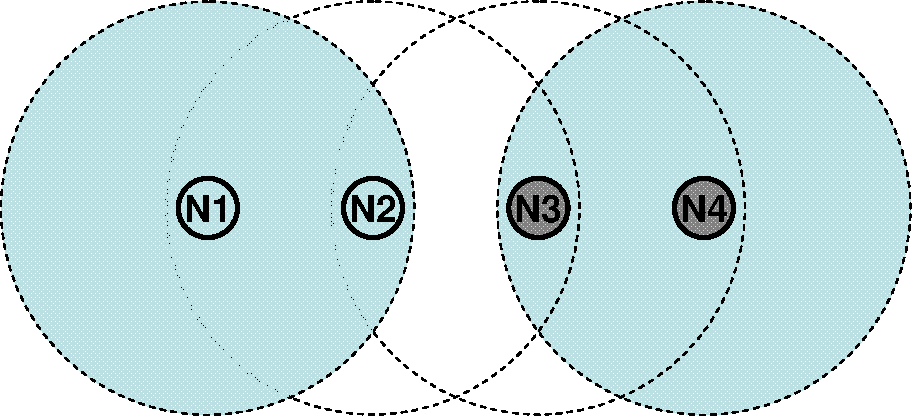
\includegraphics[width=0.6\textwidth]{Figures/four-crop.pdf} \\
\caption{A four-node wireless network, with the (idealized) coverage areas of its nodes.}
\label{f:4nodes}
\end{figure}

\paragraph{Hidden Nodes}

Consider the spontaneous wireless network represented in Figure \ref{f:4nodes}. If $N3$ agrees with its neighbours (N2 and $N4$) that it will, for the moment, have exclusive access to the wireless media via its wireless interface, then $N3$ may go ahead and make a transmission. However, if at the same time $N1$ also transmits over its wireless interface, then the transmissions of the wireless interfaces of $N1$ and $N3$ may appear concurrently at the wireless interface of $N2$ -- potentially interfering and causing $N2$ to receive neither of the transmissions. Denoted a {\em collision}, the possibility and probability of this occurring depends on the L2 (data link layer) mechanisms in place -- suffice to observe that such collisions can and do occur when using some common wireless interfaces such as IEEE 802.11. The term {\em hidden node} originates from the fact that while the node wishing exclusive access to the wireless media may negotiate this with its direct neighbours (in our case $N2$ and $N4$), nodes out of direct radio range (in our case $N1$) are {\em hidden} to the node requesting media access and cannot thus participate in the negotiation.

% (text from Thomas, from "A MANET Architecture Model", sec. 3.3)

\paragraph{Exposed Nodes}

This can be considered as the dual problem of the {\em hidden node} situation described above: an {\em exposed node} is a node that is prevented to transmit due to the transmission of a neighbor, even when the two transmissions would not be interfer. Consider again the network of Figure \ref{f:4nodes}. In the moment in which $N3$ starts a transmission, after having agreed the exclusive use of the wireless channel with neighbors $N2$ and $N4$, $N2$ is an {\em exposed node} because it is not able to transmit during the transmission of $N3$, in order to avoid collisions. Note however that not all concurrent transmissions from $N2$ would cause collision with the ongoing transmission from $N2$ to $N4$ -- in particular, there are no collisions if destinations do not receive several packets at the same time: a packet transmission from $N3$ to $N4$ and from $N2$ to $N1$ would not cause any collision. The {\em exposition} of $N2$ to the transmission of $N3$ entails thus a reduction in the available bandwidth. \ \\ \ \\
%
% (text from Thomas, from "A MANET Architecture Model", sec. 3.4)
%
The hidden and exposed node problems are consequences of the fact that links between wireless interfaces in a spontaneous wireless network are not necessarily symmetric or transitive. These are major differences with the IP networking model (see section \ref{ss:ip}), in which neighbor relationships inside an IP link are assumed to be symmetric and transitive. As these assumptions do not hold necessarily in spontaneous wireless networks, {\em wireless links in a spontaneous wireless network should not be directly modeled, in general, as IP links} \cite{softcom09}.

%{\bf Implications in addressing.-}

\subsection{An IP-compatible Architectural Model}
%\subsection{A Model for Nodes and Interfaces in Wireless Multi-Hop Ad hoc Networks}
\label{ss:model}

%This section presents the main elements of a networking model for spontaneous wireless networks and nodes \cite{tc_manetarch} that enables the compatibility of IP with the characteristics of spontaneous wireless networks. 

This section derives from the previously-described observations a general IP-compatible networking model for spontaneous wireless networks \cite{tc_manetarch}. This model enables the compatibility of IP with the characteristics of spontaneous wireless networks, without relying on assumption concerning topology or capabilities of wireless links.

\paragraph{Network View}

IP operating on a spontaneous wireless network can be conceived in two separate levels, as represented in Figure \ref{f:manetview}: the level of traditional IP networking, and the level in which wireless interfaces are connected in a spontaneous wireless network. 
\begin{itemize}
\item The first level (inner white cloud in Figure \ref{f:manetview}) contains {\em wireless interfaces} from routers that communicate with each other by way of {\em wireless links}, and form a spontaneous wireless network with the non-standard properties described throughout this section. Wireless interfaces in this level present {\em semibroadcast} communication properties (see paragraph below) and are therefore not required to satisfy the conditions of IP links. 
\item The second level (outer gray cloud in Figure \ref{f:manetview}) contains the links between routers and hosts, in which the classic IP link model, as described in section \ref{ss:ip}, applies.
\end{itemize}

%Following the architecture described in this section, a configured wireless multi-hop network with routers and hosts is splitted in two separate levels: the level of traditional IP networking, and the level in which wireless interfaces are connected in a wireless multi-hop ad hoc network. Figure \ref{f:manetview} represents this two-level structure: the inner white cloud represents the level where semibroadcast interfaces and links form a wireless multi-hop ad hoc network -- and the outer gray cloud represents the level where the classic IP link model, as described in section \ref{ss:ip}, applies.

\begin{figure}[htb]	% H-must be here or [htb]
\centering
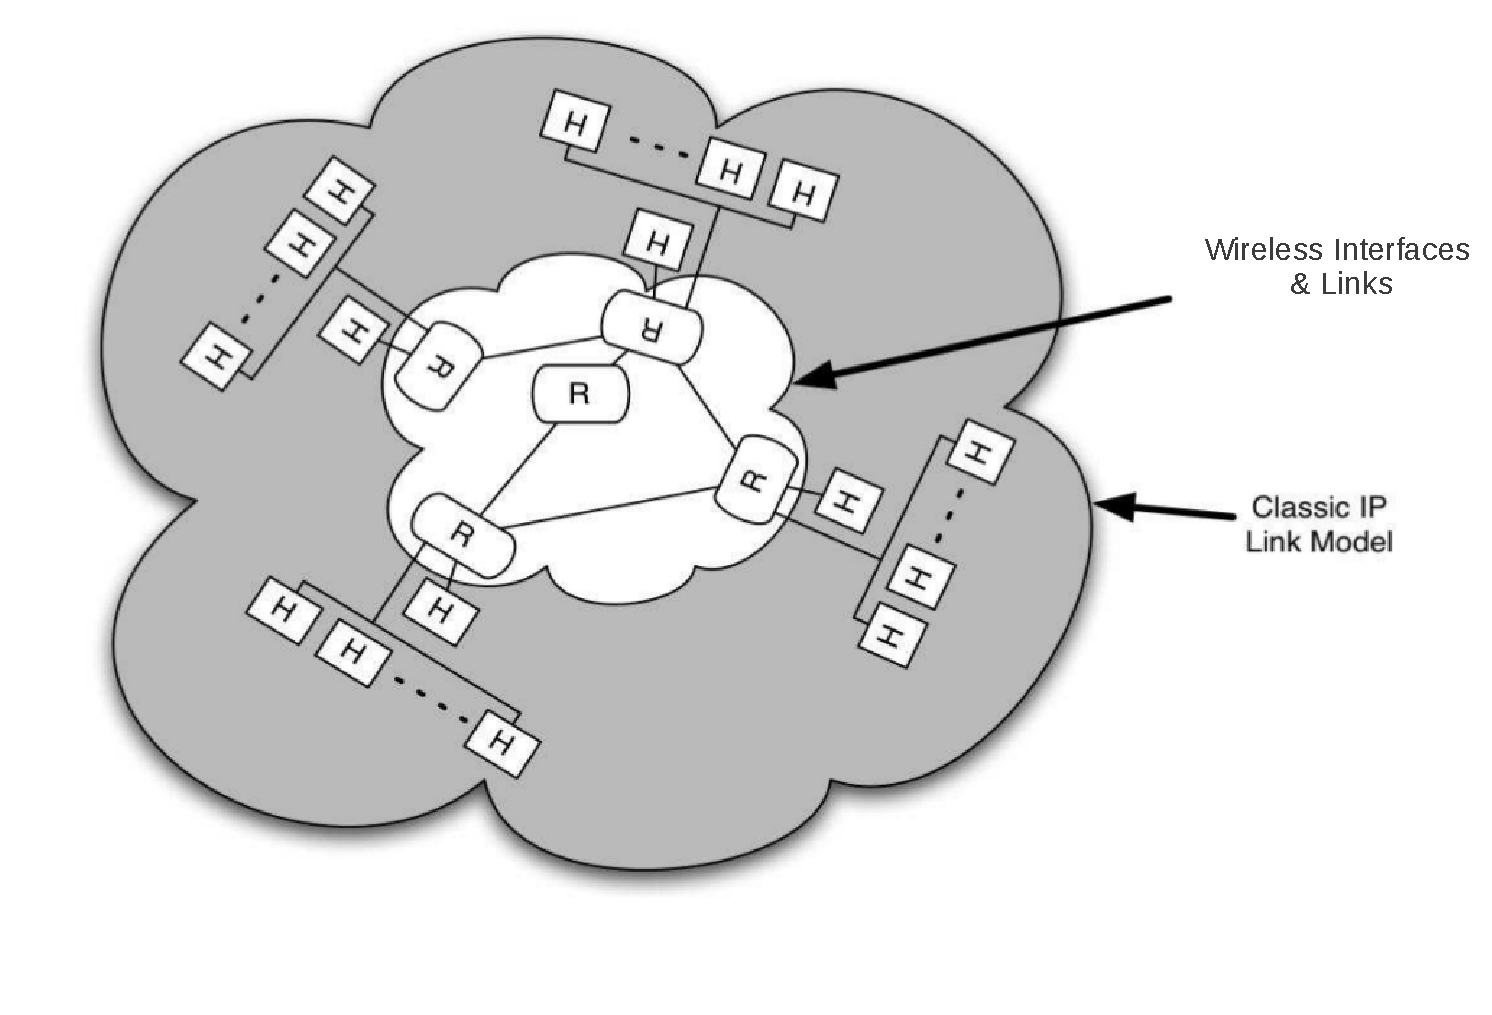
\includegraphics[width=0.75\textwidth]{Figures/manetview3-crop.pdf} \\
\caption{A view of a spontaneous wireless network, following the architecture model described in this section.}
\label{f:manetview}
\end{figure}

% (text from Thomas, from "A MANET Architecture Model", sec. 5.4)

\paragraph{Semibroadcast Interfaces}

As mentioned in section \ref{s:phy}, packets transmitted by a wireless interface $A$ are simultaneously received by the set of wireless interfaces within the coverage area of $A$, and can be successfully decoded by all those receiving interfaces for which no other transmission causes interference. In a spontaneous wireless network, this set does not contain in general all interfaces in the network. Moreover, as links are not necessarily symmetric in wireless networks and interface coverage areas have a time-variant, irregular arbitrary shape \cite{kotz03}, packets from an interface that has received and correctly decoded packets from $A$ are not guaranteed to be received and correctly decoded by $A$. Wireless {\bf semibroadcast interfaces} are thus ``broadcast-capable interfaces that {\em may} exhibit asymmetric reachability" (as defined in {\tt draft-ietf-autoconf-manetarch} \cite{ietf_manetarch}) and {\em may} not reach all interfaces in the spontaneous wireless network.

%Wireless interfaces in a wireless multi-hop ad hoc network can communicate with other interfaces (neighbors) within their coverage area. Although typically represented as a fixed radius circle around the interface (as in Figures \ref{f:cov_intf}, \ref{f:asym} and \ref{f:4nodes}), the coverage area of an interface has a time-variant, irregular arbitrary shape \cite{kotz03} -- so neighbor sets, even in a static network, are dynamic. These characteristics make possible for an interface to reach several neighboring interfaces in a single wireless transmission -- these interfaces are denominated {\bf semibroadcast interfaces} \cite{ietf_manetarch}.

%As the coverage area of different interfaces is not necessarily the same, wireless links are {\em not necessarily symmetric}: if an interface $A$ is within the coverage area of $B$, but $B$ is not included in the coverage area of $A$, then there is a link $B\longrightarrow A$, but the symmetric link $A \longrightarrow B$ does not exist. The neighborhood relationships are {\em not necessarily transitive}: the fact that an interface $A$ can communicate directly with another interface $B$, and that $B$ can communicate directly with $C$, does not imply that $A$ and $C$ can communicate directly. 

\paragraph{Node Morphology}

It has been mentioned (see section \ref{ss:spontaneous}) that nodes in a spontaneous wireless network can behave simultaneously as routers and hosts, in contrast to traditional wired computer networks which enforce a clear separation between host and router roles. A first intuition deriving from this observation leads to consider nodes in a spontaneous wireless network as standard hosts with routing capabilities, with an IP subnet prefix assigned to their wireless (semibroadcast) interfaces. This intuition however assumes implicitly that the semibroadcast interface of the router is attached to the IP link over which the host is configured (and receives its prefix), which is not consistent with the differences between IP links and links between interfaces in spontaneous wireless networks, detailed in section \ref{ss:issues}. %\ \\ \ \\
%
Instead, an alternative node model is proposed, which is compatible with the specific characteristics of links between semibroadcast interfaces, and consistent with the two-level network view described above in this subsection. In this model, a node virtually contains {\em one} router with a wireless interface to interact with the rest of wireless interfaces. As shown throughout this section, links between these wireless interfaces have semibroadcast properties and hence, cannot be configured, in general, as standard IP links in a straightforward manner. A node may also contain one or more hosts: if it does, its hosts belong to the {\em second level} of the network architecture (see Figure \ref{f:manetview}). This entails that the links between these hosts and the corresponding router are standard IP links. Figure \ref{f:node} illustrates the case of a node formed by a router $R$ with a wireless (semibroadcast) interface, and three hosts $H_1$, $H_2$ and $H_3$ connected to $R$ via standard IP links.

%As an IP link cannot be successfully built on top of a wireless multi-hop ad hoc network, as shown in section \ref{ss:issues}, this section proposes the inverse approach, that is, to build a wireless multi-hop network that connects wireless (semibroadcast) interfaces belonging to {\em nodes} that contain IP networks as described in Figure \ref{f:node}.

\begin{figure}[htb]	% H-must be here or [htb]
\centering
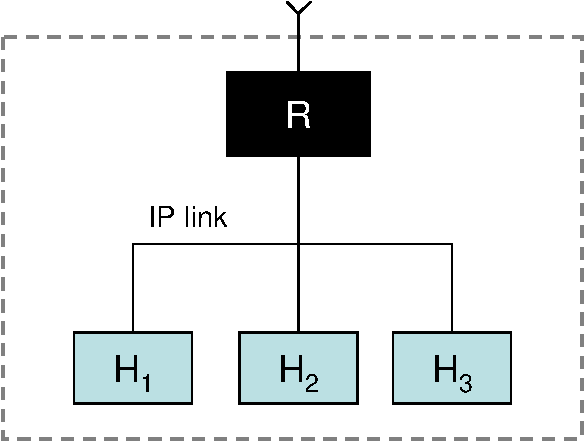
\includegraphics[width=0.35\textwidth]{Figures/manet_node-crop.pdf} \\
\caption{A node model for a spontaneous wireless network.}
\label{f:node}
\end{figure}

This implies that, from the point of view of the hosts, and the applications running on these hosts, connectivity is via a classic IP link. Host applications can thus run unaltered over spontaneous wireless networks, as the specificities of wireless semibroadcast communication have no architectural implications over the links through which hosts are connected: they remain architecturally banished to the {\em first level} depicted in Figure \ref{f:manetview}, and handled by wireless interfaces of the routers to which hosts are connected. Characteristics of multi-hop wireless communications can however still impact end-to-end performance experienced by hosts -- for instance, TCP may not be able to function as expected \cite{gerla99}. \ \\ \ \\
%
With this model, nodes in spontaneous wireless networks can behave simultaneously as hosts (that is, being source or destination of traffic) and as routers (forwarding other's traffic towards its destination), but hosts and routers interface differently with the rest of the network: hosts are connected to a classic IP link, while routers are connected to the spontaneous network by way of a semibroadcast interface over links that cannot be assumed symmetric or transitive, for instance.

%--- characteristics of wireless multi-hop ad hoc networks has no architectural effect in 

%are not exposed to the specific characteristics of the wireless semibroadcast interfaces and are connected to the wireless multi-hop network via a router, which has one or more wireless interfaces.

%This implies that, from the point of view of the hosts, and the applications running on these hosts, connectivity is via a classic IP link. Hosts, and their applications, are not exposed to the specific characteristics of the wireless semibroadcast interfaces and are connected to the wireless multi-hop network via a router, which has one or more wireless interfaces.

% (text from Thomas, from "A MANET Architecture Model", sec. 5.1)

\paragraph{Impact on IP Addressing}

IP addressing model is tied to the notion of IP link, as shown in section \ref{ss:ip}. As the assumptions underlying IP links do not hold in general on links between wireless interfaces, IP links should not be configured by default in spontaneous wireless networks \cite{rfc5889}. There are two major implications on not configuring IP links on such a network:

\begin{itemize}
\item {\bf Unique Prefixes}. Wireless interfaces must be configured with unique prefixes, {\em i.e.} such that no two wireless interfaces are configured such that they appear within the same IP subnet. Some common ways to achieve this are:

\begin{itemize}
\item unnumbered interfaces (IPv4) \cite{rfc1812};
\item Link-Local Addresses (IPv6);
\item full length prefixes: /128 (IPv6) or /32 (IPv4) prefixes.
\end{itemize}

However it is worth noting that prefix lengths shorter than /128 (IPv6) or /32 (IPv4) are possible on the semibroadcast interface, as long as the prefixes are unique to a single wireless interface.

\item {\bf Link Local Multicast/Broadcast Scope}. On a wireless interface, a Link Local multicast or broadcast reaches wireless interfaces of neighbor nodes only, regardless of their configured addresses. A Link Local multicast or broadcast on a wireless interface is, thus, a "neighborcast", and is not forwarded nor assumed to be received by all nodes within a spontaneous wireless network. \\
\end{itemize}  

% (text mostly from Thomas, from "A MANET Architecture Model", sec. 5.3)

The principles of the model described in this section have a concrete impact on spontaneous wireless networks operation as described in the remainder of the chapter. On one hand it specifies how IP interfaces should be configured on such networks, and on the other hand it identifies the need for novel protocols and the exact scope of their operation -- the {\em first level} depicted in Figure \ref{f:manetview}. The following sections will describe techniques and protocols for enabling communication at layer 3 in spontaneous wireless networks, within the scope of the {\em first level} shown in Figure \ref{f:manetview}. When needed, assumptions beyond those described in this model will be explicitly detailed in the corresponding protocols.

%\section{Flooding and Routing Mechanisms over Wireless Ad Hoc Networks}
\section{Flooding and Routing in Spontaneous Wireless Networks}
\label{s:flood_rtg}

% Note: At some point it should be clear that we are assuming a SINGLE wireless interface per router.
% Note: Provide consistent notation message/packet throughout the chapter.

As described in section \ref{s:comm_wless}, there are important differences in the way that spontaneous wireless networks enable communication between nodes, with respect to the classic fixed/wired networks. These differences have a significant impact in the mechanisms and protocols used in wireless multi-hop scenarios to disseminate information through the network ({\em flooding}) and find and maintain paths between pairs of computers in the network ({\em routing}). This section examines several mechanisms that are used in different routing protocols, discusses the issues and problems that these mechanisms have when operating in spontaneous wireless networks, and describes some techniques to fix or overcome these issues. 

Section \ref{ss:nd} explores the use of neighbor discovery procedures in spontaneous wireless networks. Section \ref{ss:flood} describes techniques to perform efficient flooding over such networks. Finally, section \ref{ss:metrics} presents the problem of estimating link costs and using them to to identify ``good routes" over the network.  

\subsection{Neighborhood Discovery}
\label{ss:nd}

In many routing and flooding protocols, routers need to be aware of their own neighborhood. This is particularly important (although not only) in spontaneous wireless networks, in which the neighborhood may change frequently during network operation. Routers acquire knowledge about their neighborhood by way of a {\bf neighborhood discovery} mechanism.

\begin{definition}[Neighborhood Discovery]
(ND) is the process whereby each router advertises all the routers to which direct communication is possible ({\em i.e.}, the routers to which there are network links) about its presence in the network. This way, routers receiving such advertisements from other (neighboring) routers gain insight on their own neighborhood.
\end{definition}

%\begin{remark}
%About "neighbor".
%Messages in which a router advertises its presence to directly-reachable routers are typically denominated {\bf Hello messages}.
%\end{remark}

\paragraph{1-hop and 2-hop neighborhood}

Depending on the information advertised by ND messages, receiving routers learn different aspects about their neighborhood. If messages only advertise the presence of the originating router, the receiving router will acquire information about the routers that maintain links to itself. If links are bi-directional (as IP links in standard IP networks), this is sufficient for enabling bi-directional communication between routers: a router receiving a ND message from a neighbor can exchange packets in both directions with it. This is the case of traditional neighbor discovery protocols for Internet, such as the \textit{Neighbor Discovery Protocol} (NDP) for IPv6 \cite{rfc4861}, which assumes that all the links are bi-directional and is used to actively keep track of which neighbors are reachable. \ \\ \ \\
%
%Neighborhood discovery is the process whereby each router discovers the routers which are in direct communication range of itself (1-hop neighbors), and detects with which of these it can establish bi-directional communication. For traditional neighbor discovery protocol for Internet, such as \textit{Neighbor Discovery in IPv6} \cite{rfc4861}, assumes that all the links are bi-directional, and is used to actively keep track of which neighbors are reachable. 
%
In spontaneous wireless networks, bi-directional communication availability cannot be inferred from the reception of an ND advertisement, given the fact that asymmetric links are possible (section \ref{ss:issues}). This is taken into account in ND protocols for spontaneous wireless networks. In these protocols, ND advertisements (typically denominated {\bf Hello messages}), contain not only the id of the originating router, but also the list of its current neighbors ({\em i.e.}, routers from which the originating router has received Hello messages). This enables every router in the network to detect the (1-hop) neighbors with which bi-directional communication is possible, and identify the routers that belong to its 2-hop neighborhood -- that is, the set of routers that are 2-hop neighbors or ``neighbors of its neighbors''. 

\begin{itemize}
\item {\bf Example} Assume that router $A$ receives a Hello from a neighbor $B$, in which $B$ indicates to have recently received a Hello from $A$; then $A$ learns that link $A$-$B$ is symmetric. As $B$ lists identifiers of all its 1-hop neighbors in its Hello, $A$ learns its 2-hop neighbors through this process.
\end{itemize}

Together with 1-hop neighbors, additional information may be included in Hello messages -- in particular, the cost of the links towards the listed neighbors, when metrics other than hop-count (see section \ref{ss:metrics}) is used. Exchange of Hello messages is typically done periodically, although some events may trigger non-periodic Hellos ({\em e.g.}, changes in the topology). \ \\ \ \\ %({\em e.g.} ETX \cite{etx}, based on the number of expected transmissions to send successfully a packet over a link, or EDR \cite{edr}, that estimates the data rate at which packets can be sent) is used.
%
The {\em Mobile Ad Hoc Network Neighborhood Discovery Protocol} (NHDP, RFC 6130) \cite{rfc6130} is the main ND protocol for spontaneous wireless networks. It is used as auxiliary protocol by other routing protocols that need neighborhood information to take their decisions, such as OLSRv2 (see section \ref{sec:olsr}). In NHDP, Hello messages are exchanged periodically and they contain the id of the originating router and the list of its 1-hop neighbors. The IETF also standardized an optimization of NDP for IPv6 over Low-Power Wireless Personal Area Networks (6LoWPANs). This optimization, specified in RFC 6775, adapts the operation of NDP to the lossy conditions of communications and the low-power device constraints of LoWPANs. This is done, for instance, by avoiding unsollicited messages (such as periodic router announcements), reducing the use of multicast for address resolution, limiting the duplicate address detection checks, or enabling better compression algorithms \cite{rfc6775}. \ \\ \ \\
%
%lossy, low-power, low-bit-rate, short-range; with many nodes saving energy with long sleep periods. Multicast as used in IPv6 Neighbor Discovery (ND) [RFC4861] is not desirable in such a wireless low-power and lossy network. Moreover, LoWPAN links are asymmetric and non-transitive in nature. 
%
Other routing protocols include their own Hello mechanism. This is the case of AODV \cite{rfc3561} (see section \ref{ss:aodv}) or OSPF and its MANET extensions \cite{rfc5449,rfc5614,rfc5820} (see section \ref{ss:ospfmanet}). In the last case, some approches have been explored in order to avoid redundant notifications and hence reduce control traffic by only reporting changes in the neighborhood occurred since the last Hello transmission: this principle leads to the {\em incremental Hellos} mechanism used in the Overlapping Relays extension of OSPF (OR/SP \cite{rfc5820}) and the {\em differential Hellos} mechanism used in the MANET Designated Routers extension of OSPF (OSPF-MDR \cite{rfc5614}). However, experiments show that the potential benefits (mostly, saved amount of traffic) of these two mechanisms are not significant, in particular when compared with the additional complexity they introduce in the corresponding protocols \cite{aircc}.

%\paragraph{ND Protocols and Optimizations for Wireless Multi-Hop Ad hoc Networks}

%The Mobile Ad Hoc Network Neighborhood Discovery Protocol (NHDP) \cite{NHDP-RFC6130} is the main ND protocol for wireless multi-hop ad hoc networks. It is used as auxiliary protocol by other routing protocols that need neighborhood information to take their decisions, such as OLSRv2. In NHDP, periodic Hello messages are exchanged locally so that each router can determine its 1-hop and symmetric 2-hop neighbors. The Hello message carries identifier of the originator, and its 1-hop neighbor information. Through Hello message exchanges, the router can determine the status of the link -- and in particular, detect whether bi-directional communication is possible: assume that router $A$ receives a Hello from a neighbor $B$, in which $B$ indicates to have recently received a Hello from $A$; then $A$ learns that link $A$-$B$ is symmetric. As $B$ lists identifiers of all its 1-hop neighbors in its Hello, $A$ learns its 2-hop neighbors through this process.

%Other routing protocols include their own Hello mechanism. This is the case of AODV \cite{AODV-RFC3561} (see section \ref{ss:aodv}) or OSPF and its MANET extensions \cite{rfc5449,rfc5614,rfc5820} (see section \ref{ss:ospfmanet}). In the last case, some optimizations have been explored in order to avoid redundant notifications by only reporting changes in the neighborhood occurred since the last Hello transmission: this principle leads to the  {\em incremental Hellos} mechanism used in the Overlapping Relays extension of OSPF (OR/SP \cite{rfc5820}) and the {\em differential Hellos} mechanism used in the MANET Designated Routers extension of OSPF (OSPF-MDR \cite{rfc5614}). However, experiments show that the potential benefits of these two mechanisms are not very relevant, in particular when compared with the additional complexity they introduce in the corresponding protocols \cite{aircc}.

 %Each router sends Hellos, listing the identifiers of all the routers from which it has recently received a Hello, as well as the ``status'' of the link (heard, verified bi-directional). 

%The purpose of the Hello message is to broadcast the local node topology information to the one-hop neighbors to serve the task such as link sensing and neighbor detection.

\subsection{Flooding}
\label{ss:flood}
%
Flooding is the process through which information originated in one router is disseminated across the network, so that it can be received by every other router in the network. \ \\ \ \\
%
The most obvious procedure to perform flooding from a router in a conventional IP network consists of the {\bf pure flooding} procedure:

\begin{enumerate}
\item The source router sends the message through all its network interfaces.
\item Every router that receives the message {\em for the first time} retransmits it over all the network interfaces {\em except the one over which it was received}.
\end{enumerate}

The fact that each router retransmits only {\em once} ensures that the process terminates in a finite number of steps. The fact that {\em all} routers receiving the message retransmit it ensures that the message is received --if there are no packet losses-- by every router in the network at least once. \ \\ \ \\
%
In a spontaneous wireless network, as routers communicate with {\em all} their wireless neighbors by way of a {\em single} wireless interface (see section \ref{s:comm_wless}), the straightforward usage of this mechanism implies that the source router broadcasts the message to be flooded and the neighboring routers rebroadcast it over the same interface it was received. It is known \cite{broadcaststorm} that such a naive approach is not efficient and does not scale in a wireless multi-hop scenario. Three reasons can be highlighted: 

\begin{enumerate}[a)]
\item excessive retransmissions that reduce the available bandwidth, 
\item systematic packet collisions due to concurrent transmissions of wireless interfaces (partly) sharing the same wireless channel, and 
\item duplicate packets reception due to the fact that the packet is received and retransmitted over the same interface (and, therefore, transmitted twice in the intersection between the coverage area of the sender and the receiver interface). 
\end{enumerate}

\begin{remark}
Although the three effects are closely inter-related, and all are due to the bandwidth scarcity and the semi-broadcast properties of wireless communication detailed in section \ref{s:comm_wless}, it is important to point out that they constitute {\em different} effects; solving one of them does not necessarily solve the others. 
\end{remark}

\paragraph{Excessive Number of Retransmissions and Efficient Flooding}

In a spontaneous wireless network, a single transmission from a wireless interface is received by the wireless interfaces of all the neighbors within its coverage area. If all routers retransmit the same message as they receive it, this is likely to cause a significant number of {\em redundant transmissions} -- {\em i.e.}, transmissions that do not bring new information for {\em any} of the interfaces receiving them. \ \\ \ \\
%
Consider the situation in Figure \ref{f:excessive}, in which node $A$ (in the center) floods a message to all its neighbors, and they in turn retransmit the same message so that it is received by all the 2-hop neighbors of $A$. In theory, every 2-hop neighbor has received the message -- possibly several times. The redundant retransmissions do not bring new information, but increase the probability of collisions. This effect becomes more relevant in a context of bandwidth scarcity and high network router density. %, as node $C_2$ which receives it from $B_1$, $B_2$ and $B_3$. Some retransmissions of $A$'s 1-hop neighbors are {\em redundant}, for instance $B_2$: if $B_2$ had not retransmitted the message, all the 2-hop neighbors that received $B_2$'s retransmission ($C_1$, $C_2$ and $C_3$) would have received the message via $B_1$ and $B_3$. In practice, the situation is worse: as several transmissions are being performed at the same time by close nodes that share (at least partly) the same wireless channel, the probability of packet collisions is high: several 2-hop neighbors "theoretically" covered by different 1-hop neighbors may be in practice unable to receive and decode successfully the message from $A$, due to collisions between retransmitters \cite{broadcaststorm}. 

\begin{figure}[h]
\centering
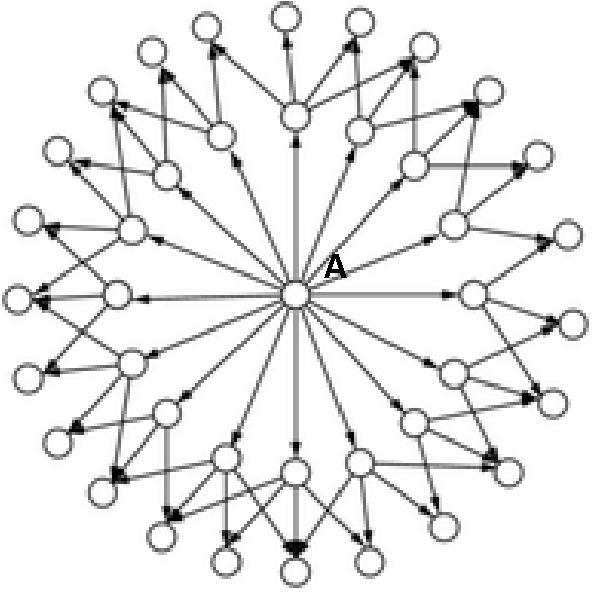
\includegraphics[width=0.4\textwidth]{Figures/purebc-crop.pdf}
\caption{Classical flooding in spontaneous wireless networks.}
\label{f:excessive}
\end{figure}

{\bf Efficient flooding} techniques explore different strategies to reduce the number of flooding retransmissions (and therefore, to decrease the amount of traffic overhead involved), while preserving as much as possible the ability of the flooding procedure to reach all (or most of) the routers in the spontaneous wireless network. \ \\ \ \\
%
For every efficient routing technique, a set of the routers that receive a message (typically, not all of them) are allowed to retransmit it. If efficient flooding reaches all routers in the network, the set of routers allowed to retransmit a message is a {\em Dominating Set} (DS) in the network graph. As only one router originates and originally sends the message, and every other forwarding router has previously received it via flooding, the set of routers and the wireless links between them usually form a {\bf Connected Dominating Set} (CDS). Given a graph $G=(V,E)$ representing a spontaneous wireless network, where $V$ is the set of vertices (representing network routers) and $E$ is the set of edges (representing network links), a Connected Dominating Set of $G$ is a subset of vertices $D \subseteq V$ with two properties:

%, assuming that the message is originally sent by only one router and every other forwarding router has received the message previously

\begin{enumerate}
\item {\em Connection}. $D$ induces a connected subgraph of $G$, that is, any node in $D$ can reach any other node in $D$ by a path that stays entirely within $D$. 
	\begin{align*}
	\forall x, y \in V &,& \exists p=(x, p_1, p_2, ..., p_n, y) \subseteq D \wedge \bar{xp_1}, \bar{p_1p_2}, ..., \bar{p_ny} \in E
	\end{align*}
\item {\em Domination}. $D$ is a dominating set of $G$, meaning that every vertex in $G$ either belongs to $D$ or is adjacent to a vertex in $D$.
	\begin{align*} 
	\forall v \in V &,& v \in D \vee ( \exists w \in D : \bar{uw} \in E )
	\end{align*}
\end{enumerate} 

%The rules used for determining which routers are selected as {\em flooding relays} lead to different techniques \cite{broadcaststorm}.

Figure \ref{f:ex_cds} displays an example of Connected Dominating Set over a network graph.

\begin{figure}[htb]	% H-must be here or [htb]
\centering
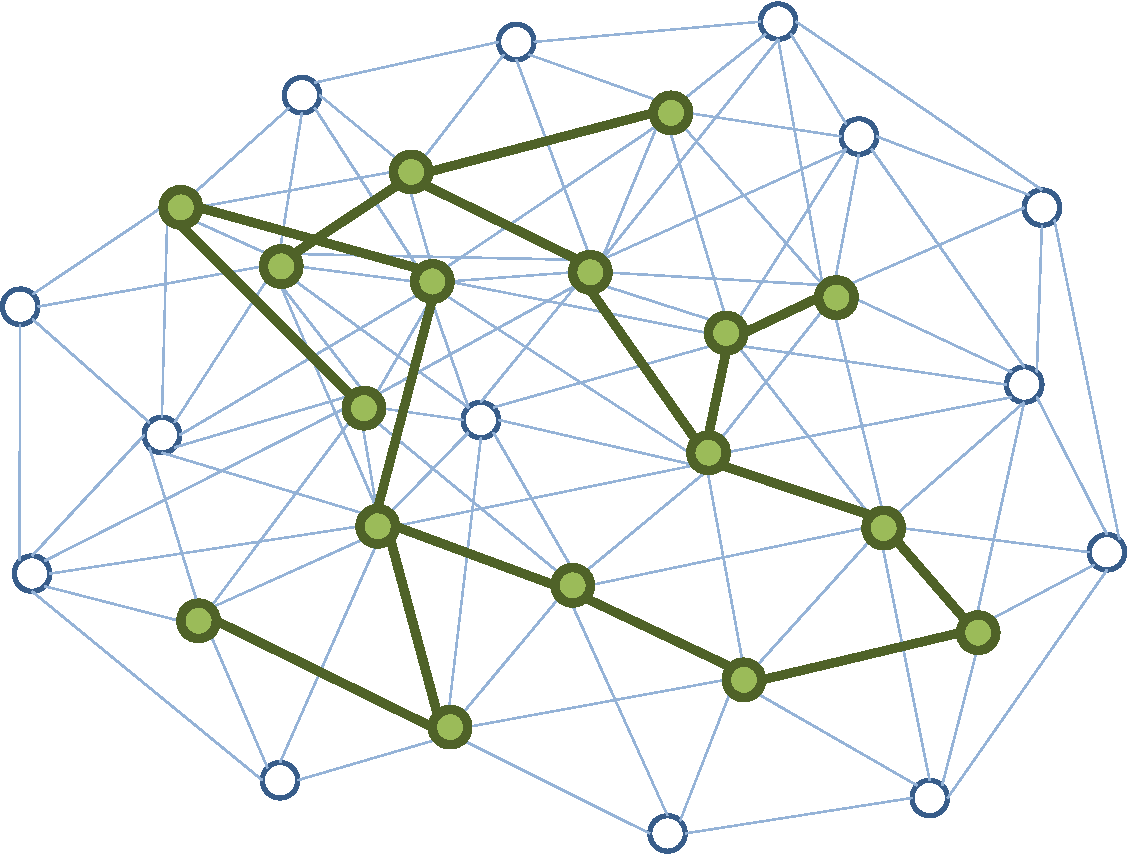
\includegraphics[width=0.6\textwidth]{Figures/excds-crop.pdf} %	** if .eps or .pdf, don't need extension}
\caption{Example of CDS (thick edges) over a network graph of 30 nodes (light edges represent communication between nodes).}
\label{f:ex_cds}
\end{figure}

The notion of CDS is useful for efficient flooding purposes: several efficient flooding techniques rely on the construction and maintenance of Connected Dominating Sets of forwarding nodes, over which packets are flooded through the network. One of the main techniques based on this principle is the {\em Multi-Point Relaying} (MPR) technique.

\begin{itemize}
\item {\bf Multi-Point Relays} \cite{mpr-hicss2002} is an algorithm through which a node selects a subset of its 1-hop neighbors (\emph{multi-point relays}) such that each 2-hop neighbor is reachable through (at least) one of the selected 1-hop neighbors ({\em MPR coverage criterion}). MPR selection requires that the selecting node knows the 2-hop neighbors that will be covered by its MPRs. By using MPR, the retransmission of flooding traffic can be significantly reduced, as shown in Figure \ref{f:mpr}, compared to classical flooding in Figure \ref{f:excessive}. 

\begin{figure}[h]
\centering
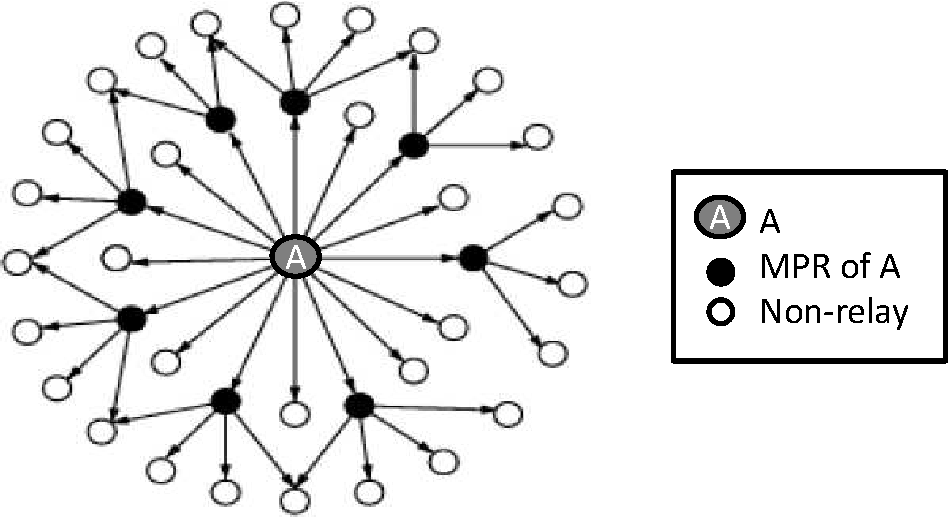
\includegraphics[width=0.65\textwidth]{Figures/mpr-crop.pdf}
\caption{Efficient flooding with Multi-Point Relays.}
\label{f:mpr}
\end{figure}

	\begin{remark}
	Note that the MPR coverage criterion does not guarantee by itself that the set of nodes selected as MPRs form a Connected Dominating Set \cite{softcom10}. The set of MPRs is by definition a dominating set, as every node is either a MPR for a neighbor, or is adjacent to its own MPR. As the heuristic for MPR selection is relative to the source, however, the subgraph resulting from MPRs and the MPR links (links connecting nodes with their relays) between them {\em is not necessarily connected}. This can be easily fixed by adding an arbitrary router and all its links to the subgraph, as proved in Cordero (2010) \cite{softcom10}.
	\end{remark}

%\begin{itemize}
%\item We present MPR: MPR, by which each router is able to, efficiently, conduct network-wide broadcasts. Each router designates, from among its bi-directional neighbors, a subset (MPR set) such that a message transmitted by the router and relayed by the MPR set is received by all its 2-hop neighbors
%\end{itemize}

Multipoint relays of a router can be used to perform efficient flooding, but the principle can be used for performing other networking operations. The MPR selection algorithm can be slightly modified so that the overlay that includes all links between routers and its (modified) multi-point relays is sufficient to compute shortest paths over the underlying network \cite{softcom10}. This result has been exploited in some extensions of OSPF for MANETs, as shown in section \ref{s:wospf}.

\end{itemize}

%The idea behind different kind of efficient flooding techniques is to find a reduced CDS. One of these techniques is the {\bf Multi-Point Relaying} (MPR) technique.


\paragraph{Systematic Packet Collisions and Jittering Techniques}

Consider the spontaneous wireless network of Figure \ref{f:syspcol}, in which router $A$ floods a message through the network. The broadcast transmission of $A$ is received at the same time by $B$ and $C$, which retransmit the message towards $E$ and $D$ (in the case of $B$) and $D$ and $F$ (in the case of $C$). Then, concurrent retransmissions from $B$ and $C$ cause a systematic packet collision from $D$'s perspective.

\begin{remark}
In this example, the collision could not be detected with any CSMA\footnote{Carrier Sense Multiple Access. CSMA is a medium access control (MAC) protocol for wireless networks in which nodes sense the medium before transmitting, and only transmit if the sensed medium is idle, that is, if the node does not detect any ongoing transmission within its reception range. See {\em e.g.} Tanenbaum {\em et al.} \cite{tanenbaum} for reference.} layer 2 mechanism neither by $B$ nor by $E$, due to the fact that $B$ and $E$ are not neighbors to each other. $B$ is a {\em hidden node} for $E$ (and vice versa).
\end{remark}

\begin{remark}
Note that this problem cannot be addressed only by way of {\em efficient flooding} approaches: none of the retransmissions by $B$ and $E$ are redundant, so none of them could be avoided without leaving nodes uncovered ($C$ if $B$ does not retransmit, $F$ if $E$ does not retransmit). 
\end{remark}

\begin{figure}
\centering
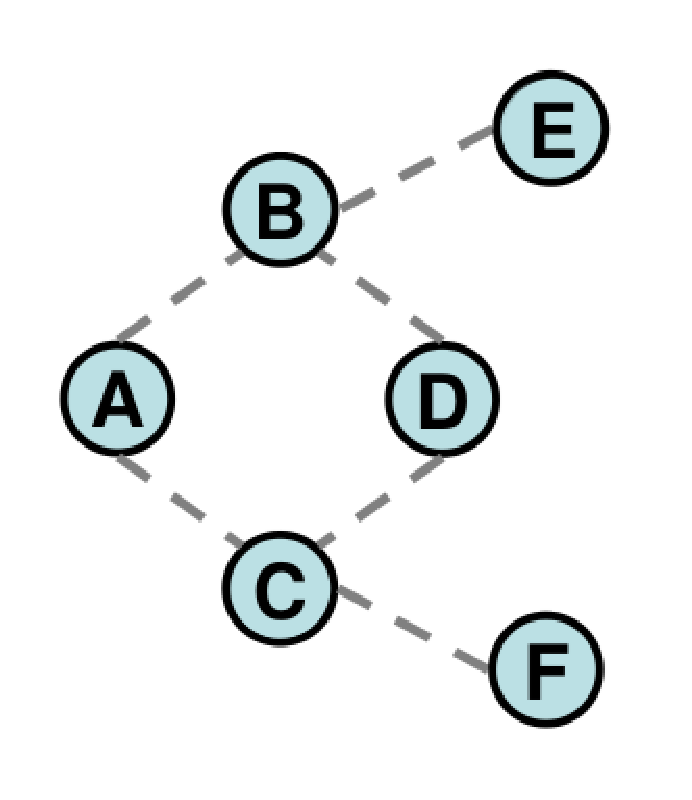
\includegraphics[width=0.2\textwidth]{Figures/abcdef-crop.pdf}
\caption{An example of spontaneous wireless network. {\em (Broken lines denote direct communication)}}
\label{f:syspcol}
\end{figure}

The fact that flooded messages are forwarded simultaneously by wireless interfaces receiving them through the same wireless shared medium may cause packet collisions during the flooding procedure (depending on the network topology at the time of flooding). Unlike other packet transmissions for which the collision probability may vary depending on the traffic pattern, these flooding collisions are {\em systematic} and will occur, for a given network topology and flooding algorithm, any time that the source node floods a new message (in the example, any time $A$ floods a message). \ \\ \ \\
%
This effect could be alleviated by allowing routers to wait a random amount of time (denominated {\bf jitter}) before retrasmitting a flooded message, in order to reduce the probability of concurrent transmissions by neighboring wireless interfaces. This technique is known as {\bf jittering}, and has been standardized by the IETF in RFC 5148 \cite{rfc5148}. The recommendation from RFC 5148 is that delays are selected following an uniform distribution between $0$ and a maximum jitter value, $MAX\_JITTER$. Figure \ref{f:jitter} illustrates the effect of jittering techniques in the network example of Figure \ref{f:syspcol}. In the example, node \textit{A} is flooding a packet to all the other nodes. When node \textit{B} and \textit{C} receive the packet from \textit{A}, instead of retransmitting the packet immediately, they wait a random delay. In this way, simultaneous transmission of $B$ and $C$ (which can cause collision at $D$ in this case) can be avoided. \ \\ \ \\
%
\begin{figure}[htb]
\centering
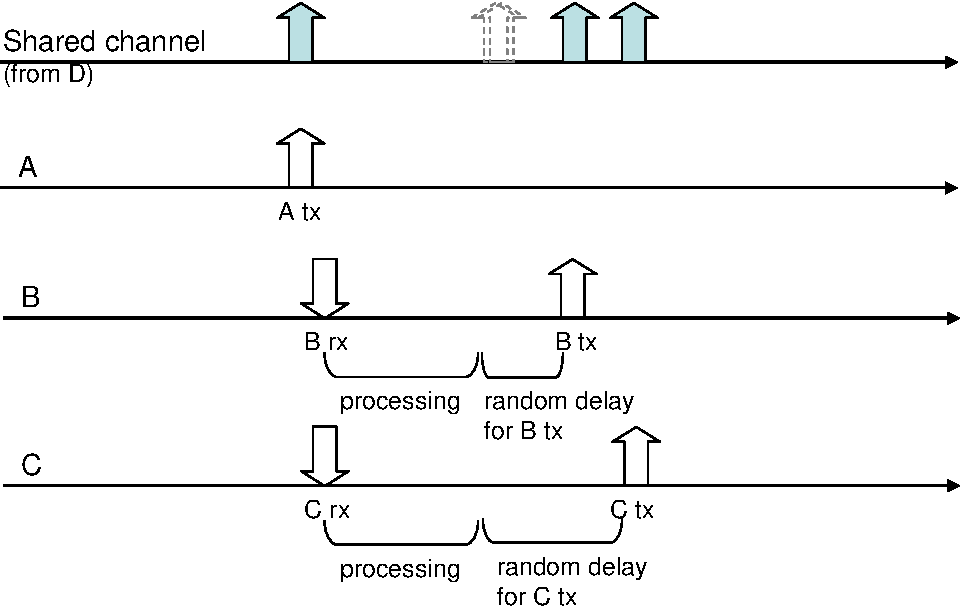
\includegraphics[width=0.6\textwidth]{Figures/jitter4flooding-crop.pdf}
\caption{Use of jitter for flooding. Node \textit{A} is flooding a packet in a network. Node \textit{B} and \textit{C} wait a random delay before the packet is retransmitted. The dashed overlapping arrows represent the packet collision that would occur if no jitter were used.}
\label{f:jitter}
\end{figure}
%
Although jittering can be theorically implemented at different layers of the protocol stack, it has been shown that its use in layers upper than L3 brings little benefit \cite{jitter-broadcast}. As the problem of systematic collisions affects every L3 routing protocol using wireless flooding, jittering techniques can be implemented by different protocols. The addition of random delays in flooded packets impacts differently in proactive and reactive protocols, given the different use of flooding in both routing strategies. Other jittering effects are due to the specifities of the techniques employed in each case. In proactive protocols where jitter is used (as described in RFC 5148 \cite{rfc5148}, which recommends to introduce random delays and piggyback all pending messages when a transmission is scheduled), such as OLSR or the OSPF extensions for MANETs, jittering leads to longer LSA messages -- this may cause additional packet collisions, if jitter values are not configured properly \cite{INFOCOM-jitter,jitter-wpc}. In reactive protocols such as AODV, where jitter is used for Route Request (RREQ) flooding, the addition of random delays may lead to suboptimal path selections, which can be minimized by adapting the random distribution used for determining jitter values \cite{Infocom12, wiopt}.  

\paragraph{Duplicate Packets and Detection Techniques}

The reception of duplicate packets is a common situation in wireless flooding, due to the fact that flooded messages are retransmitted by forwarding nodes over the same wireless interface in which they were received. Consider the situation of Figure \ref{f:dpd}: router \textit{N2} is retransmitting a broadcast packet received from router \textit{N1} on the same interface as the one over which it was received, so as to ensure receipt also by router \textit{N3}, causing router \textit{N1} to receive the packet a second time.

\begin{figure}[ht]
\centering
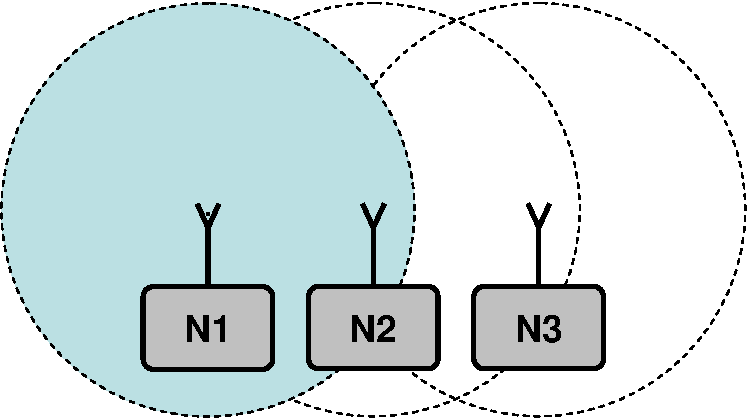
\includegraphics[width=0.4\textwidth]{Figures/dpd.pdf}
\caption{The need for duplicate detection: retransmission over the same interface as a packet was received.}
\label{f:dpd}
\end{figure}

Depending of the protocol and the use it makes of flooding and of flooded packets, the way to detect duplicate packets might be different. In link-state routing protocols such as OLSR or OSPF, for instance, flooded messages are link-state advertisements (LSAs) that are stored locally before being retransmitted, in case they bring fresh topology information; in this case, a duplicate LSA can be easily recognized by checking whether the LSA is already installed in the local Link-State Database (LSDB). If flooded messages are not stored locally, the protocol needs to store state for every forwarded message in order to detect a duplicate -- this is, for instance, the strategy of the Simplified Multicast Forwarding (SMF) protocol \cite{rfc6621}. In case a received message was already received and forwarded, it is dropped.

%\subsection{Synchronization}
\subsection{Link Metrics}
\label{ss:metrics}

\glslink{metric}{Metrics} are used to evaluate the cost of a link or a path (set of links), so that a routing protocol is able to determine whether a path or a link should be preferred over another. \ \\ \ \\
%
The simplest link \glslink{metric}{metric} is the {\bf hop-count}: a link has \glslink{metric}{metric} 1 if it is available, 0 otherwise. Typically, in the early versions of routing protocols for spontaneous wireless networks (e.g., AODV, OLSRv1 for mobile ad hoc networks), only the hop-count \glslink{metric}{metric} is used. This way, the \glslink{metric}{metric} or cost for a path is equal to the number of hops involved. \ \\ \ \\
%
When a route between two hosts is being calculated under the hop-count metric, paths with less number of hops are preferred to paths with more number of hops. However, using only minimum hop routes in spontaneous wireless networks may result in suboptimal routing in practice, as the minimum-hop routes are not necessarily the best ones \cite{couto03, wang95}. \ \\ \ \\
%
Figure \ref{f:metric} give an example showing the limit of hop-count metric. The minimum hop route from node \textit{A} to \textit{B} is $\{A,X,B\}$. However, the links $\bar{AX}$ and $\bar{XB}$ are poor with high loss rate (but still able to deliver packets), and $\bar{AY}$, $\bar{YZ}$, $\bar{ZB}$ are reliable links. In this case, $\{A,Y,Z,B\}$ is preferred to the route with minimum hop count. \ \\ \ \\
%
\begin{figure}
\centering
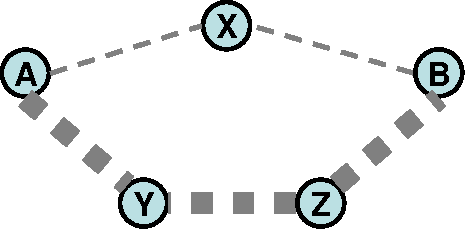
\includegraphics[width=0.25\textwidth]{Figures/axb-crop.pdf}
\caption{An example of different link metric. $\bar{AX}$, $\bar{XB}$ are unreliable links; $\bar{AY}$, $\bar{YZ}$, $\bar{ZB}$ are reliable links.}
\label{f:metric}
\end{figure}
%
Because of the limitation of hop-count metric, new metrics need to be defined. The link metrics used in spontaneous wireless network are expected to have following properties \cite{metrics}:

\begin{itemize}
\item {\bf Dimensionless}. The \glslink{metric}{metric} may correspond to specific physical information, but this knowledge is not used by the routing protocol. 
\item {\bf Additiveness}. The \glslink{metric}{metric} of a route is the sum of the metrics of the links forming that route. It also requires a \glslink{metric}{metric} where a low value of a link \glslink{metric}{metric} indicates a "good" link a high value of a link \glslink{metric}{metric} indicates a ``bad" link. 
\item {\bf Directionality}. The \glslink{metric}{metric} from a router $A$ to router $B$ does not need be the same as the \glslink{metric}{metric} from $B$ to $A$. This is a direct consequence of the fact that wireless links are not bi-directional. 
\end{itemize}

The kind of \glslink{metric}{metric} used in a network depends on the link/physical layer protocol used, the type of information that is available from lower layers, the application requirements, etc. Some examples of link \glslink{metric}{metric} include delay, packet loss probability (Expected Transmission Count, ETX \cite{etx}, that estimates the average number of transmissions before success over a link), queue length (at the receiver) or data rates (Expected Data Rate, EDR \cite{edr}; this \glslink{metric}{metric} is not additive, thus a mapping that inverts its ordering must be applied).

%%\begin{itemize}
%%\item Delay. 
%%\item Packet loss probability. 
%%\item Queue length. 
%%\item Data rates. It is not additive, thus a mapping that inverts its ordering must be applied. 
%%\end{itemize}

%\section{Specific Flooding and Routing Protocols for Wireless Multi-Hop Ad hoc Networks}
\section{IETF Routing Protocols for Spontaneous Wireless Networks}
\label{s:specific}
%
Since the late 1990s, in parallel with the emergence and deployment of new and more flexible networking technologies, the IETF has embarked upon a path of designing, developing and standardizing new routing protocols and flooding mechanisms. These protocols and mechanisms are designed for networks with increasingly more fragile and low-capacity links, with less pre-determined connectivity properties and with increasingly constrained router resources. \ \\ \ \\
%
Most of the IETF protocol design and standardization activity has focused on protocols designed for Mobile Ad hoc Networks (MANETs) and Low-Power Lossy Networks (LLNs), both defined in section \ref{ss:manet_lln}. This section presents the main flooding and routing protocols designed and standardized by the IETF for these types of networks in the last years: OLSRv1 and OLSRv2, RPL, AODV and LOADng.
%
\paragraph{Routing in MANETs: OLSR and AODV}
%
IETF activities targeting MANETs have converged on the development of two protocols, each one representative of one of the two main routing families (see section \ref{ss:routing}): reactive and proactive routing. \ \\ \ \\
%
IETF design and standardization work in the reactive routing realm for mobile ad hoc networks first led to the Ad-hoc On-demand Distance Vector protocol (AODV) \cite{rfc3561}; the efforts in proactive routing, in turn, led to the Optimized Link State Routing (OLSR) \cite{rfc3626}. A distance vector protocol, AODV operates in an \textit{on-demand} fashion, acquiring and maintaining routes only while needed for carrying data, by way of \textit{Route Request}-\textit{Route Reply} exchanges. A link state protocol, OLSR is based on periodic control messages exchanges, and each router proactively maintaining a routing table with entries for all destinations in the network. OLSR provides low delays in forwarding and has a predictable, constant control overhead -- at the expense of requiring memory in each router for maintaining complete network topology. AODV limits the memory required for routing state to that for actively used routes -- at the expense of delays for the \textit{Route Request}-\textit{Route Reply} exchange to take place, and control overhead dependent on data flows. \ \\ \ \\
%
Based on the operational experience acquired through AODV and OLSRv1, the IETF is currently designing and developing successors for OLSR and AODV. In the first case, the IETF community involved in OLSR has standardized OLSR version 2 (OLSRv2) \cite{OLSRv2} and its related components (packet format \cite{rfc5444} \cite{rfc5497}, NHDP \cite{rfc6130}). Work on AODV version 2 \cite{ietf:aodvv2} has started, as AODV derivative flourished: IEEE 802.11s \cite{IEEE-802.11s-principles}, which is based on AODV, and the G3-PLC standard \cite{itu:PLC-G3}, published in 2011, which specifies the use of the {\em 6LoWPAN Ad hoc Routing Protocol} (LOAD, specified in {\tt draft-daniel-6lowpan-adhoc-routing}) \cite{ietf:I-D:LOAD} at the MAC layer, for providing layer 2 routing for utility (electricity) metering networks. 
%
\paragraph{Routing in LLNs: RPL and LOADng}
%
LLNs can be regarded as a subset of MANETs, but with more stringent constraints in terms of device CPU and memory limitations, and work over more fragile links. Concerning LLNs, two protocols can be highlighted: RPL and LOADng. The IETF explored the problems of routing and adaptation of IPv6 for operation over the IEEE 802.15.4 MAC protocol, accommodating characteristics of that MAC layer, and with a careful eye on resource constrained devices (memory, CPU, energy, ...). Two initial approaches to such routing were explored: {\em mesh-under} and {\em route-over}. Both approaches entail different additional assumptions on the (link) characteristics of the addressed spontaneous wireless network, not present in the general networking model described in section \ref{ss:model}.
	\begin{enumerate}
	\item The {\em mesh-under} approach performs L2.5 multi-hop routing, that is, provides routing in an adaptation layer between 802.15.4 (MAC layer, L2) and IP (network layer, L3). This L2.5 routing enables the underlying mesh-routed multi-hop topology to be presented at the network layer as a single broadcast domain.
	\item The {\em route-over} approach, in contrast, exposes the underlying multi-hop topology to the IP layer, whereupon IP routing would build multi-hop connectivity. 
	\end{enumerate}
The IETF efforts on routing over 802.15.4 initially led to LOAD \cite{ietf:I-D:LOAD}, a derivative of AODV adapted for L2-addresses and mesh-under routing, and with some simplifications over AODV (\eg~removal of intermediate node replies and sequence numbers). However, 6LoWPAN was addressing other issues regarding adapting IPv6 for IEEE 802.15.4, such as IP packet header compression, and efforts to solve routing issues were suspended. In parallel with these efforts, the IETF has also specified the ``Routing Protocol for Low-power lossy networks'' (RPL), designed to support 6LoWPAN networks in a route-over configuration \cite{rfc6550, rpl-ipso}. \ \\ \ \\
%
However, reasons for using a simplified reactive approach instead of RPL have emerged, including better support for bi-directional data flows such as a request/reply of a meter reading \cite{RPL-bidirectional}, as well as algorithmic and code complexity reasons \cite{RPL-criticism}. These observations led on one hand to a renewed interest in AODV-derived protocols for specific scenarios, resulting in LOADng \cite{ietf:I-D:LOADng} \cite{ietf:I-D:LOADng-interop} and AODVv2 \cite{ietf:aodvv2}, while on the other hand leading to the development of an extension of RPL to support reactive path discovery (P2P-RPL \cite{ietf:rpl-p2p}).
%
% However, 6LowPAN was addressing other issues regarding adapting IPv6 for IEEE 802.15.4, such as IP packet header compression, and solving the routing issues was suspended, delegated to a working group ROLL, created in 2008 for this purpose. ROLL produced a routing protocol denoted ``Routing Protocol for Low-power lossy networks'' (RPL)  \cite{ietf:RFC6550:RPL} in 2012.
%
%Part of the original charter for this working group was to develop protocols for routing in multi-hop topologies under such constrained conditions, and over this particular MAC. Two initial philosophies to such routing were explored: {\em mesh-under} and {\em route-over}. The former, mesh-under, would, as part of an adaptation layer between 802.15.4 and IP, provide L2.5 multi-hop routing, presenting an underlying mesh-routed multi-hop topology as a single IP link. The latter, route-over, would expose the underlying multi-hop topology to the IP layer, whereupon IP routing would build multi-hop connectivity. Several proposals for routing were presented in 6LowPAN, for each of these philosophies, including LOAD \cite{ietf:I-D:LOAD}. LOAD was a derivative of AODV, but adapted for L2-addresses and mesh-under routing, and with some simplifications over AODV (\eg~removal of intermediate node replies and sequence numbers). However, 6LowPAN was addressing other issues regarding adapting IPv6 for IEEE 802.15.4, such as IP packet header compression, and solving the routing issues was suspended, delegated to a working group ROLL, created in 2008 for this purpose. ROLL produced a routing protocol denoted ``Routing Protocol for Low-power lossy networks'' (RPL) \cite{ietf:RFC6550:RPL} in 2012.
%
%Justifications for using an AODV derivative in preference to RPL include that the former better supports bi-directional data flows such as a request/reply of a meter reading \cite{RPL-bidirectional}, as well as algorithmic and code complexity reasons \cite{RPL-criticism}. The emergence of LLNs thus triggered a renewed interest in AODV-derived protocols for specific scenarios, resulting in work within the IETF \cite{ietf:I-D:LOADng} and \cite{ietf:I-D:LOADng-interop} for the purpose of standardization of  LOADng, incorporating the experiences from deploying AODV -- including, but not only, in LLNs.
%
%Since the late 1990s, the IETF has embarked upon a path of developing routing protocols for networks with increasingly more fragile and low-capacity links, with less pre-determined connectivity properties and with increasingly constrained router resources. In '97, by chartering the MANET working group, then subsequently in 2006 and 2008 by chartering the 6LowPAN and ROLL working groups.
%
%\paragraph{MANET Protocol Developments}
%The MANET working group converged on the development of two protocol families: reactive protocols, including AODV  \cite{AODV-RFC3561}, and proactive protocols, including  Optimized Link State Routing (OLSR) \cite{OLSR-RFC3626}.  A distance vector protocol, AODV operates in an \textit{on-demand} fashion, acquiring and maintaining routes only while needed for carrying data, by way of a \textit{Route Request}-\textit{Route Reply} exchange. A link state protocol, OLSR is based on periodic control messages exchanges, and each router proactively maintaining a routing table with entries for all destinations in the network, which provides low delays but constant control overhead.  A sizable body of work exists, including \cite{SIMCOMP}, studying the performance of these protocols in different scenarios, and justifying their complementarity \cite{LIX-NET-journal-1}.  OLSR provides low delays and predictable, constant control overhead -- at expense of requiring memory in each router for maintaining complete network topology. AODV limits the memory required for routing state to that for actively used routes -- at the expense of delays for the \textit{Route Request}-\textit{Route Reply} exchange to take place, and control overhead dependent on data flows.
%
%After acquiring operational experiences, the MANET working group commenced developing successors to OLSR and AODV, denoted OLSRv2 and DYMO. Whereas a relatively large and active community around OLSR thus standardized OLSRv2 \cite{jitter-RFC5148}, \cite{packetbb-RFC5444}, \cite{tlv-RFC5497}, \cite{NHDP-RFC6130} and \cite{OLSRv2}, the momentum behind DYMO withered in the MANET working group\footnote{http://tools.ietf.org/wg/manet/minutes?item=minutes81.html}.
%
%In the meantime, AODV derivative live on: IEEE 802.11s \cite{IEEE-802.11s-principles} is based on AODV, and the G3-PLC standard  \cite{itu:PLC-G3}, published in 2011, specifies the use of \cite{ietf:I-D:LOAD} at the MAC layer, for providing mesh-under routing for utility (electricity) metering networks. Justifications for using an AODV derivative in preference to RPL include that the former better supports bi-directional data flows such as a request/reply of a meter reading \cite{RPL-bidirectional}, as well as algorithmic and code complexity reasons \cite{RPL-criticism}. The emergence of LLNs thus triggered a renewed interest in AODV-derived protocols for specific scenarios, resulting in work within the IETF \cite{ietf:I-D:LOADng} and \cite{ietf:I-D:LOADng-interop} for the purpose of standardization of  LOADng, incorporating the experiences from deploying AODV -- including, but not only, in LLNs.
%
%\paragraph{6LowPAN and ROLL Protocol Developments}
%
%The 6LowPAN working group was chartered for adapting IPv6 for operation over IEEE 802.15.4, accommodating characteristics of that MAC layer, and with a careful eye on resource constrained devices (memory, CPU, energy, ...). Part of the original charter for this working group was to develop protocols for routing in multi-hop topologies under such constrained conditions, and over this particular MAC. Two initial philosophies to such routing were explored: {\em mesh-under} and {\em route-over}. The former, mesh-under, would, as part of an adaptation layer between 802.15.4 and IP, provide L2.5 multi-hop routing, presenting an underlying mesh-routed multi-hop topology as a single IP link. The latter, route-over, would expose the underlying multi-hop topology to the IP layer, whereupon IP routing would build multi-hop connectivity. Several proposals for routing were presented in 6LowPAN, for each of these philosophies, including LOAD \cite{ietf:I-D:LOAD}. LOAD was a derivative of AODV, but adapted for L2-addresses and mesh-under routing, and with some simplifications over AODV (\eg~removal of intermediate node replies and sequence numbers). However, 6LowPAN was addressing other issues regarding adapting IPv6 for IEEE 802.15.4, such as IP packet header compression, and solving the routing issues was suspended, delegated to a working group ROLL, created in 2008 for this purpose. ROLL produced a routing protocol denoted ``Routing Protocol for Low-power lossy networks'' (RPL)  \cite{ietf:RFC6550:RPL} in 2012.
%
\subsection{Optimized Link State Routing Protocol (OLSR)}
\label{sec:olsr}
%
OLSR is developed for mobile ad hoc networks, and operates as a  table driven, proactive protocol, i.e., it exchanges topology information with other routers in the network regularly. The key concept used in the protocol is that of multipoint relays (MPRs, described in section \ref{ss:flood}), selected nodes which forward broadcast messages during the flooding process. This efficient flooding technique substantially reduces the message overhead as compared to a classical flooding mechanism. \ \\ \ \\
%
OLSR version 1 was standardized in RFC 3626 \cite{rfc3626}. The work continues as OLSR version 2 (OLSRv2 \cite{OLSRv2}), which retains the same basic algorithms as its predecessor, however offers various improvements, {\em e.g.} a modular and flexible architecture allowing extensions, such as security, to be developed as add-ons to the basic protocol. \ \\ \ \\
%
%(new)
Every router running OLSR in the network generates two types of messages: {\em Hellos} and {\em Topology Control} (TC) messages. Information collected through exchange of these messages allows routers to perform the three basic processes of OLSR: Neighborhood Discovery, Link State Advertisements and Routing Set Calculation. Because OLSR (version 1) and OLSRv2 shares the same basic mechanisms, the text below applies to both protocols. 
%
%\paragraph{Routing Control Messages}\label{sec:olsr-msg}
%
%Every router running OLSR in the network generates two types of messages: Hellos and TC (Topology Control), to exchange topology information of the network. 
%
%\begin{itemize}
%\item {\bf Hello messages}. Hello messages are exchanged between a router and its 1-hop neighbors for neighbor discovery purposes, as explained in section \ref{ss:nd}. They can be generated proactively at a regular interval or as a response to a change in the router itself. In OLSR, a Hello message contains the local interface address(es), and its 1-hop neighbor addresses. With the broadcast of Hello messages to the router's 1-hop neighbor, the router is able to get the topology information in two hops. 
%\item {\bf Topology Control (TC) messages}. TC messages are broadcast by each node to the whole network to build the intra-forwarding database needed for routing packets. A TC message is sent by a node in the network to declare a set of links, which must include at least the links to all nodes of its MPR Selector set, {\em i.e.}, the neighbors which have selected the sender node as a MPR. TC messages are flooded to all nodes in the network and take advantage of MPRs. MPRs enable a better scalability in the distribution of topology information. With the broadcast of TC messages to the whole network, the node is able to get the topology information that is more than two hops away.
%\end{itemize}
%
\paragraph{Neighborhood Discovery}
%
OLSR routers discover their neighborhood by exchanging Hello messages with their 1-hop neighbors, as explained in section \ref{ss:nd}. These Hello messages can be generated proactively at a regular interval or as a response to a change in the router itself. In OLSR, a Hello message contains the local interface address(es), and its 1-hop neighbor addresses. With the broadcast of Hello messages to the router's 1-hop neighbor, the router is able to get the topology information in two hops.
%
%Hello messages are exchanged between a router and its 1-hop neighbors for neighbor discovery purposes, as explained in section \ref{ss:nd}. They can be generated proactively at a regular interval or as a response to a change in the router itself. In OLSR, a Hello message contains the local interface address(es), and its 1-hop neighbor addresses. With the broadcast of Hello messages to the router's 1-hop neighbor, the router is able to get the topology information in two hops.
%
\paragraph{Link State Advertisements}
%
%TC messages are broadcast by each node to the whole network to build the intra-forwarding database needed for routing packets. A TC message is sent by a node in the network to declare a set of links, which must include at least the links to all nodes of its MPR Selector set, {\em i.e.}, the neighbors which have selected the sender node as a MPR. TC messages are flooded to all nodes in the network and take advantage of MPRs. MPRs enable a better scalability in the distribution of topology information. With the broadcast of TC messages to the whole network, the node is able to get the topology information that is more than two hops away.
%
Link State Advertisement is the process where by the determined link state information is advertised through the network. For OLSR, this process is optimized by MPR flooding. MPR selection is encoded in outgoing Hellos. \ \\ \ \\
%
% JACF: Jiazi, I replaced the "planned" term for "managed", with a small explanation (as requested by reviewers). Is the notion correct?
Routers may express, in their Hello messages, their ``willingness'' (integer between 1 ``will never'' and 7 ``will always'') to be selected as MPR, which is taken into consideration for the MPR calculation. This is useful, for example, when an OLSRv2 network is {\em managed}, meaning that its topology is known or predictable. The set of routers having selected a given router as MPR is the MPR-selector-set of that router.  Each router must advertise, at least, all links between itself and its MPR-selector-set, in order to allow all routers to calculate shortest paths. \ \\ \ \\
%
Such link state advertisements are carried in Topology Control (TC) messages. TC messages are broadcast by each node to the whole network to build the intra-forwarding database needed for routing packets. A TC message is sent by a node in the network to declare a set of links, which must include at least the links to all nodes of its MPR Selector set, {\em i.e.}, the neighbors which have selected the sender node as a MPR. TC messages are received by all nodes in the network, by way of the MPR flooding process described above. With the broadcast of TC messages to the whole network, the node is able to get the topology information that is more than two hops away. TCs are sent periodically, however certain events may trigger non-periodic TCs.
%
%MPRs enable a better scalability in the distribution of topology information.
%
% broadcast through the network using the MPR flooding process described above. As a router selects MPRs only from among bi-directional neighbors, links advertised in TC are also bi-directional and routing paths calculated by OLSRv2 contain only bi-directional links. 
%
%Each router must advertise, at least, all links between itself and its MPR-selector-set, in order to allow all routers to calculate shortest paths. Such link state advertisements are carried in Topology Control (TC) messages, broadcast through the network using the MPR flooding process described above. As a router selects MPRs only from among bi-directional neighbors, links advertised in TC are also bi-directional and routing paths calculated by OLSRv2 contain only bi-directional links. TCs are sent periodically, however certain events may trigger non-periodic TCs.
%
\paragraph{Routing Set Calculation}
%
The Routing Set of a router is populated with Routing Tuples that represent paths from that router to all destinations in the network.  These paths are calculated based on the Network Topology Graph, which is constructed from information in the Information Bases, obtained via Hello and TC message exchange. \ \\ \ \\
%
Changes to the Routing Set do not require any messages to be transmitted.  The state of the Routing Set should, however, be  reflected in the IP routing table by adding and removing entries from that routing table as appropriate.  Only appropriate Routing Tuples  (in particular only those that represent local links or paths to routable addresses) need to be reflected in the IP routing table. \ \\ \ \\
%
OLSR does not mandate which algorithm to be used for path calculation, as along as the shortest paths for all destinations from all local OLSR interfaces can be obtained using Network Topology Graph. One example is Dijkstra's algorithm \cite{dijkstra59}. 
%
\subsection{Ad Hoc On-Demand Distance-Vector Protocol (AODV)}
\label{ss:aodv}
%
The Ad hoc On-Demand Distance Vector (AODV) \cite{rfc3561} protocol enables dynamic, self-starting, multi-hop routing between participating mobile  routers wishing to establish and maintain an ad hoc network.  AODV allows mobile nodes to obtain routes quickly for new destinations,  and does not require nodes to maintain routes to destinations that  are not in active communication. \ \\ \ \\
%
Compared to pro-active protocols like OLSR, AODV is more suitable under following constraints:
%
\begin{itemize}
\item Few concurrent traffic flows in the network (i.e., traffic flows only between few sources and destinations);
\item Little data traffic overall, and therefore the traffic load from periodic signaling (for proactive protocols) is greater than the  traffic load from flooding RREQs (for reactive protocols);
\item State requirements on the router are very stringent, i.e., it is beneficial to store only few routes on a router.
\end{itemize}
%
AODV was initially standardized as an experimental RFC in 2003 \cite{rfc3561}. Derivatives of AODV include 802.11s (with HWMP \cite{IEEE-802.11s-principles}) and LOADng \cite{ietf:I-D:LOADng}. In the following of this section, the basic mechanisms of AODV, \textit{Route Discovery} and \textit{Route Maintenance} are explained. Then a main derivative work of AODV, called LOADng, is also introduced. Note that at the time of writing, work on AODVv2 \cite{ietf:aodvv2} has just started, and thus we will not elaborate further on AODVv2 in this chapter.
%
\paragraph{Route Discovery}
%
The route discovery process is initiated when a source router needs a route to a destination router and it does not have a route in its routing table. The source router floods the network with a RREQ packet specifying the destination for which the route is requested. When the destination router, or an intermediate router with sufficiently up-to-date information about the requested destination, receive the RREQ packet, they generate a Route Reply (RREP) packet, which is sent back to the source along the reverse path. Each router along the reverse path sets up a forward pointer to the router it received the RREP from. This sets up a forward path from the source to the destination.
%
\paragraph{Route Maintenance}
%
When a router detects a broken link while attempting to forward a packet to the next hop, it generates a RERR packet that is sent to all sources using the broken link. The RERR packet erases all routes using the link along the way. If a source receives a RERR packet and a route to the destination is still required, it initiates a new route discovery process.
%
\subsubsection{Lightweight On-demand Ad hoc Distance-Vector (LOADng)}
%\subsubsection{Lightweight On-demand Ad hoc Distance-Vector Protocol (LOADng)}
%
The {\em Lightweight On-demand Ad hoc Distance-vector Routing Protocol - Next Generation} (LOADng) \cite{ietf:I-D:LOADng} is derived from AODV. Compared to AODV \cite{rfc3561}, it has more concise and flexible message format, and simplified message processing, which makes it more adapted to networks with constrained devices, such as sensor networks. It is also used for ITU Standard G. 9956 \cite{itu:PLC-G3}. \ \\ \ \\
%
Compared to AODV, LOADng has both simplifications and extensions to be more suitable to LLNs:
%
\begin{itemize}
\item Only the destination is permitted to respond to an RREQ;  intermediate LOADng Routers are explicitly prohibited from responding to RREQs, even if they may have active routes to the  sought destination. This also eliminates Gratuitous RREPs while  ensuring loop freedom, so that the protocol complexity can be greatly reduced. %, and RREQ/RREP messages generated by a given  LOADng Router share a single unique, monotonically increasing sequence number.  This also eliminates Gratuitous RREPs while  ensuring loop freedom.  The rationale for this simplification is  reduced complexity of protocol operation and reduced message sizes.
\item A LOADng Router does not maintain a precursor list, thus when forwarding of a data packet to the recorded next hop on the route  to the destination fails, an RERR is sent only to the originator  of that data packet.  The rationale for this simplification is an  assumption that few overlapping routes are in use concurrently in  a given network.
\item Optimized flooding is supported, reducing the overhead incurred by  RREQ generation and flooding.  If no optimized flooding operation  is specified for a given deployment, classical flooding is used by default.
\item Different address lengths are supported -- from full 16 bytes IPv6 addresses over 6 bytes MAC addresses and 4 bytes IPv4 addresses to shorter 1 and 2 bytes addresses such as RFC 4944 \cite{rfc4944}.  The only requirement is, that within a given routing domain, all addresses are of the same address length.
\item Control messages are carried by way of the Generalized MANET Packet/Message Format \cite{rfc5444}. 
\item  Using RFC 5444 \cite{rfc5444}, control messages can include TLV (Type-Length-Value) elements, permitting protocol extensions to be developed.
\item LOADng supports routing using arbitrary additive metrics, which can be specified as extensions to this protocol.
\end{itemize}
%
%\subsubsection{802.11s: Routing in Layer 2}
%
%IEEE 802.11s is an IEEE amendment for mesh networking, which defines how wireless devices can interconnect to create a wireless mesh network. Unlike usual IP routing protocols that work in Layer 3 (Network Layer), IEEE 802.11s performs Layer 2 (Link Layer) routing. In some context, it is called ``mesh-under" routing. \ \\ \ \\
%
%To provide basic interoperability, and also extensibility, IEEE 802.11s provides several options:
%
%\paragraph{HWMP (Hybird Wireless Mesh Protocol)}
%HWMP is  the default routing protocol for IEEE 802.11s. It is the minimum requirement to provide interoperability. The foundation of HWMP is an adaptation of AODV called RM-AODV (Radio-Metric AODV). It works in layer 2 with MAC addresses and uses a radio-aware routing metric, instead of hop-count metric. 
%
%\paragraph{RA-OLSR}
%
%RA-OLSR (Radio-Aware OLSR) is an optional proactive routing protocol in 802.11s, which is based on OLSR. 
%
%\paragraph{Vendor specific extensions}
%
%IEEE 802.11s provides also an extensible framework that allows the use of other routing protocols and/or routing metrics that are better adapted in different scenarios. However, only one can be active in a 802.11s network at a time. 
%
\subsection{Routing Protocol for LLNs (RPL)}
%
RPL -- the {\em Routing Protocol for Low Power and Lossy Networks}  \cite{rfc6550} -- is an IPv6 routing protocol designed and standardized by the ROLL Working Group in the IETF. It is is intended to be the IPv6 protocol for LLNs and sensor networks, applicable in all kinds of deployments and applications of LLNs.
% 
\paragraph{DODAG Construction}
%
The basic construct in RPL is a ``Destination Oriented Directed Acyclic Graph'' (DODAG), depicted in Figure \ref{f:dodag} . In a converged LLN, each RPL router has identified a stable set of parents, each of which is a potential next-hop on a path towards the ``root'' of the DODAG, as well as a preferred parent. Each router, which is part of a DODAG (i.e. has selected parents) will emit DODAG Information Object (DIO) messages, using link-local multicast, indicating its respective rank in the DODAG (i.e. distance to the DODAG root according to some metric(s), in the simplest form hop-count). Upon having received a (number of such) DIO messages, a router will calculate its own rank such that it is greater than the rank of each of its parents, select a preferred parent and then itself start emitting DIO messages. The emission of DIO message is controlled by \textit{Trickle} Algorithm \cite{rfc6206}, to reduce the flooding overhead. \ \\ \ \\
%
\begin{figure}[ht]	
\centering
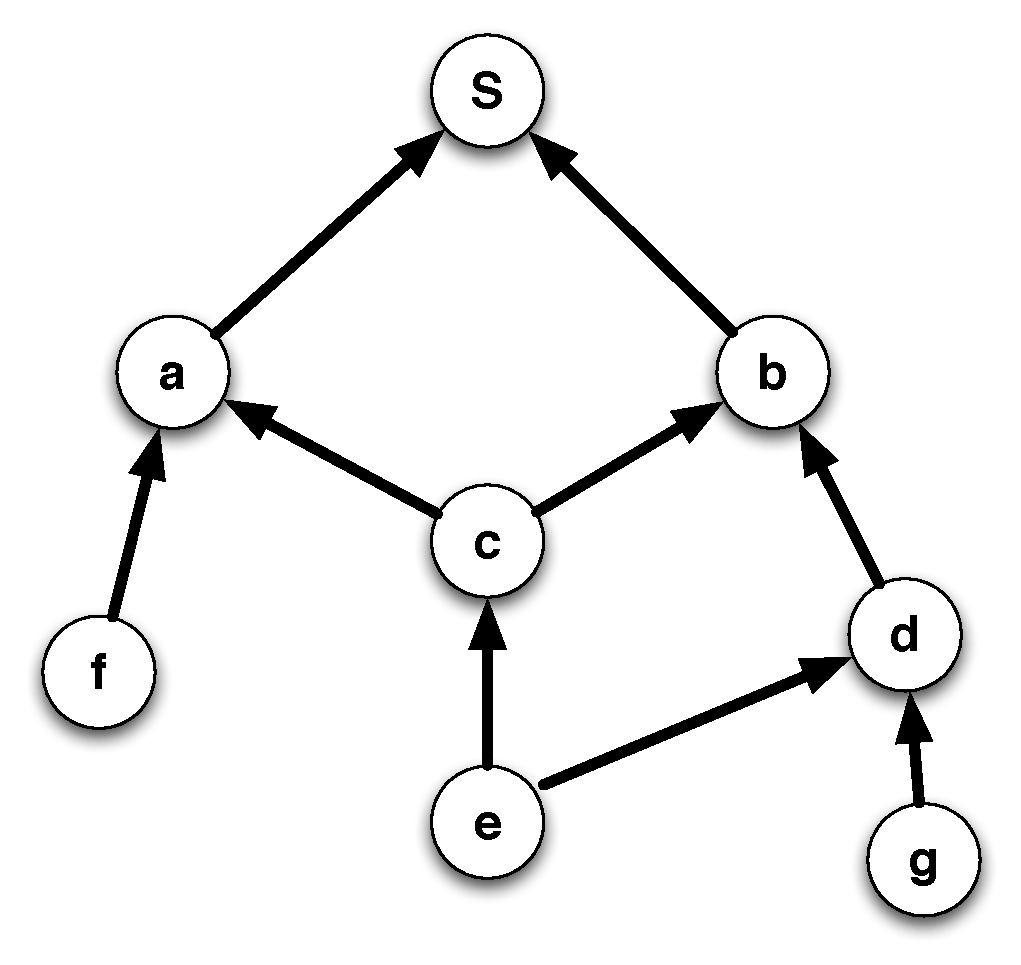
\includegraphics[width=0.3\textwidth]{Figures/Example_1.pdf}
\caption{RPL Basic Construct: DODAGs}
\label{f:dodag}
\end{figure}
%
The DODAG formation thus starts at the DODAG root (initially, the only router which is part of a DODAG), and spreads gradually to cover the whole LLN as DIOs are received, parents and preferred parents are selected and further routers participate in the DODAG. The DODAG root also includes, in DIO messages, a DODAG Configuration Object, describing common configuration attributes for all RPL routers in that network - including their mode of operation, timer characteristics etc. RPL routers in a DODAG include a verbatim copy of the last received DODAG Configuration Object in their DIO messages, permitting also such configuration parameters propagating through the network. \ \\ \ \\
%
A Distance Vector protocol, RPL restricts the ability for a router to change rank. A router can freely assume a smaller rank than previously advertised (i.e. logically move closer to the root) if it discovers a parent advertising a lower rank, and must then disregard all previous parents of higher ranks. The ability for a router to assume a greater rank (i.e. logically move farther from the root) than previously advertised is restricted, to avoid count-to-infinity problems. The root can trigger ``global recalculation" of the DODAG by increasing a sequence number, DODAG version, in DIO messages. \ \\ \ \\
%
The DODAG so constructed is used for installing routes: the ``preferred parent'' of an RPL router can serve as a default route towards the root, or the root can embed in its DIO messages the destination prefixes, included by DIOs generated by RPL routers through the LLN, to which connectivity is provided by the root. Thus, RPL by way of DIO generation provides ``upward routes'' or ``multipoint-to-point routes'' from the sensors inside the LLN and towards the root. \ \\ \ \\
%
``Downward routes'', i.e., the routes from root to sensor nodes, are enabled by having sensors issue Destination Advertisement Object (DAO) messages, propagating as unicast via parents towards the DODAG root. These describe which prefixes belong to, and can be reached via, which RPL router. In a network, all RPL routers must operate in either of storing-mode or non-storing-mode, specified by way of a ``Mode of Operation'' (MOP) flag in the DODAG Configuration Object from the root. Depending on the MOP, DAO messages are forwarded differently towards the root:
%
\begin{itemize}
\item In \textit{non-storing-mode}, an RPL router originates DAO messages, advertising one or more of its parents, and unicast it to the DODAG root. Once the root has received DAOs from an RPL router, and from all routers on the path between it and the root, it can use source routing for reaching advertised destinations inside the LLN.

\item In \textit{storing-mode}, each RPL router on the path between the originator of a DAO and the root records a route to the prefixes advertised in the DAO, as well as the next-hop towards these (the router, from which the DAO was received), then forwards the DAO to its preferred parent.

\end{itemize}
%
``Point-to-point routes'', for communication between devices inside the LLN and where neither of the communicating devices are the DODAG root, are as default supported by having the source sensor transmit via its default route to the DODAG root (i.e., using the upward routes) which will then, depending on the ``Mode of Operation'' for the DODAG, either add a source-route to the received data for reaching the destination sensor (downward routes in non-storing-mode) or simply use hop-by-hop routing (downward routes in storing-mode). In the case of storing-mode, if the source and the destination for a point-to-point communication share a common ancestor other than the DODAG root, a downward route may be available (and used) before reaching the DODAG root. Both of these modes stretch the route by important factors, and lead to significantly longer paths compared to the shortest P2P paths available in the network \cite{nbis2010}. To address this issue, an extension of RPL called RPL-P2P \cite{ietf:rpl-p2p} is currently developed by the IETF. P2P-RPL defines a new mode of operation which provides RPL with a reactive approach to discover better paths on demand between an arbitrary source and destination, without having to go through the root or the first common ancestor of this source and destination.\ \\ \ \\
%
%\subsubsection{RPL Message Emission Timing - Trickle Timers}
%
%\subsubsection{RPL Discussion}
%
While RPL has been specified as \textit{Proposed Standard} in IETF, its applicability and performance in LLNs are not yet fully understood \cite{rpl-observation}. The following lists some limitations and concerns that have emerged concerning basic RPL mechanisms.
%
\paragraph{Requirement of DODAG Root}
%
In RPL, the DODAG Root has both a special responsibility and is subject to special requirements. The DODAG Root is responsible for determining and maintaining the configuration parameters for the DODAG, and for initiating DIO emissions. The DODAG Root is also responsible (in both storing and non-storing mode) for being able to, when downward routes are supported, maintain sufficient topological information to be able to construct routes to all destinations in the network.\ \\ \ \\
%
In a given deployment, selected RPL Routers can be provisioned with the required energy, memory and computational resources so as to serve as DODAG Roots, and be administratively configured as such - with the remainder of the RPL Routers in the network being of typically lesser capacity. In storing mode, the DODAG root needs to keep a routing entry for all RPL Routers in the RPL instance. In non-storing mode, the resource requirements on the DODAG Root are likely much higher than in storing mode, as the DODAG Root needs to store a network graph containing complete routes to all destinations in the RPL instance, in order to calculate the routing table (whereas in storing mode, only the next hop for each destination in the RPL instance needs to be stored, and aggregation may be used to further reduce the resource requirements).
%
\paragraph{Data Traffic Flows}
%
RPL makes a-priori assumptions of data traffic types, and explicitly defines three such traffic types: 
%
\begin{enumerate}
\item sensor-to-root data traffic (multipoint-to-point), which is predominant, 
\item root-to-sensor data traffic (point-to-multipoint), which is rare, and 
\item sensor-to-sensor (point-to-point) data traffic, which is extremely rare.
\end{enumerate} 
%
RPL is suited for networks where sensor-to-root traffic is dominant, by distribution of DIO messages and building of a collection tree. The one way traffic from the sensor to the root can be forwarded through the preferred parent. \ \\ \ \\
%
However, the data traffic characteristics, assumed by RPL, do not represent a universal distribution of traffic types in LLNs. There are scenarios where sensor-to-sensor traffic is a more common occurrence, e.g., in Building Automation scenarios. In addition, there are scenarios, where all traffic is bi-directional. For example, the IETF protocol for use in constrained environments, CoAP \cite{CoAP1,CoAP2}, makes use of acknowledgments to control packet loss and ensure that packets are received by the packet destination. In the four message types defined for CoAP: confirmable, acknowledgement, reset and non-confirmable, the first three are dedicated for sending/acknowledgement cycle.
%
\paragraph{The DAO Mechanisms: Downward and Point-to-Point Routes}
%
In RPL, the ``mode of operation" stipulates that either downward routes are not supported (MOP=0), or that they are supported by way of either storing or non-storing mode. In case downward routes are supported, RPL does not provide any mechanism for discriminating between which routes should or should not be maintained. In particular, in order to calculate routes to a given destination, all intermediaries between the DODAG Root and that destination must themselves be reachable – effectively rendering downward routes in RPL an ``all-or-none" situation. \ \\ \ \\
%
The basic mechanisms in RPL force the choice between requiring all RPL Routers to have sufficient memory to store route entries for all destinations (storing mode)� or suffer increased risk of fragmentation, and thus loss of data packets, while consuming network capacity by way of source routing through the DODAG Root (non-storing mode). \ \\ \ \\
%
In addition, RPL does not explicitly specify how the DAO message are sent, which are used to build ``downward'' routes from root to sensors. This would make the different implementations unlikely to be interoperable. 
%
%\subsection{Simplified Multicast Forwarding (SMF)}
%\label{ss:smf}
%
%Simplified Multicast Forwarding \cite{rfc6621} is developed by IETF, which provides basic IP multicast routing for MANETs. It is mainly applicable in situations where efficient flooding represents an acceptable engineering design trade- off. It consists of two main components: multicast {\em Duplicate Packet Detection} (DPD) and {\em Relay Set Selection} (RSS). 
%
%\paragraph{Duplicate Packet Detection} DPD is used as part of the forwarding process to check if an incoming packet has been previously received (and forwarded) --and therefore should be dropped-- or not. This is achieved, as mentioned in section \ref{ss:flood}, by maintaining a record of recently processed multicast packets, and comparing received multicast packets herewith. A duplicate packet detected is silently dropped and not inserted into the forwarding path of that router, nor delivered to an application.
%
%As proposed by SMF, DPD supports both IPv4 and IPv6 and for each suggests two duplicate packet detection mechanisms: 
%
%\begin{itemize}
%\item  header content identification-based DPD (I-DPD), using packet headers, in combination with flow state, to estimate temporal uniqueness of a packet. 
%\item  hash-based DPD (H-DPD), employing hashing of selected header fields and payload for the same effect.
%\end{itemize} 
%
%\paragraph{Relay Set Selection} RSS is used in SMF to produce a reduced relay set for use when relaying information across the MANET. An efficient reduced relay set is constructed by selecting and  updating, as needed, a subset of all possible routers in a MANET   routing domain to act as SMF forwarders.  Known distributed relay set  selection algorithms have demonstrated the ability to provide and maintain a dynamic connected set for forwarding multicast IP packets. 
%
%SMF supports the use of several relay set algorithms, including ECDS (Essential Connected Dominating Set), S-MPR (Sourcebased Multi-Point Relay), or MPR-CDS. Those algorithms are based on localized election, derived from those explored for efficient topology diffusion in MANET routing protocols.
%
%\subsubsection{Duplicate Packet Detection}
%
%\subsubsection{Relay Set Selection}

\section{Routing in Wired/Wireless Internetworks with OSPF}
\label{s:wospf}
%
Protocols reviewed in section \ref{s:specific} have been specifically designed for spontaneous wireless networks. However, the increasing deployment of wireless technologies and the integration of different sorts of flexible networks with the Internet is leading to more complex inter-networks, neither purely wired networks nor purely spontaneous wireless networks, resulting from the interconnection of wireless mesh networks with fixed, wired networking infrastructure, inside Internet's Autonomous Systems. Figure \ref{f:cpd_as} shows schematically a {\em compound Autonomous System}, in which fixed and wireless mesh networks are interconnected in the same routing domain. \ \\ \ \\
%
\begin{figure}[h]
\centering
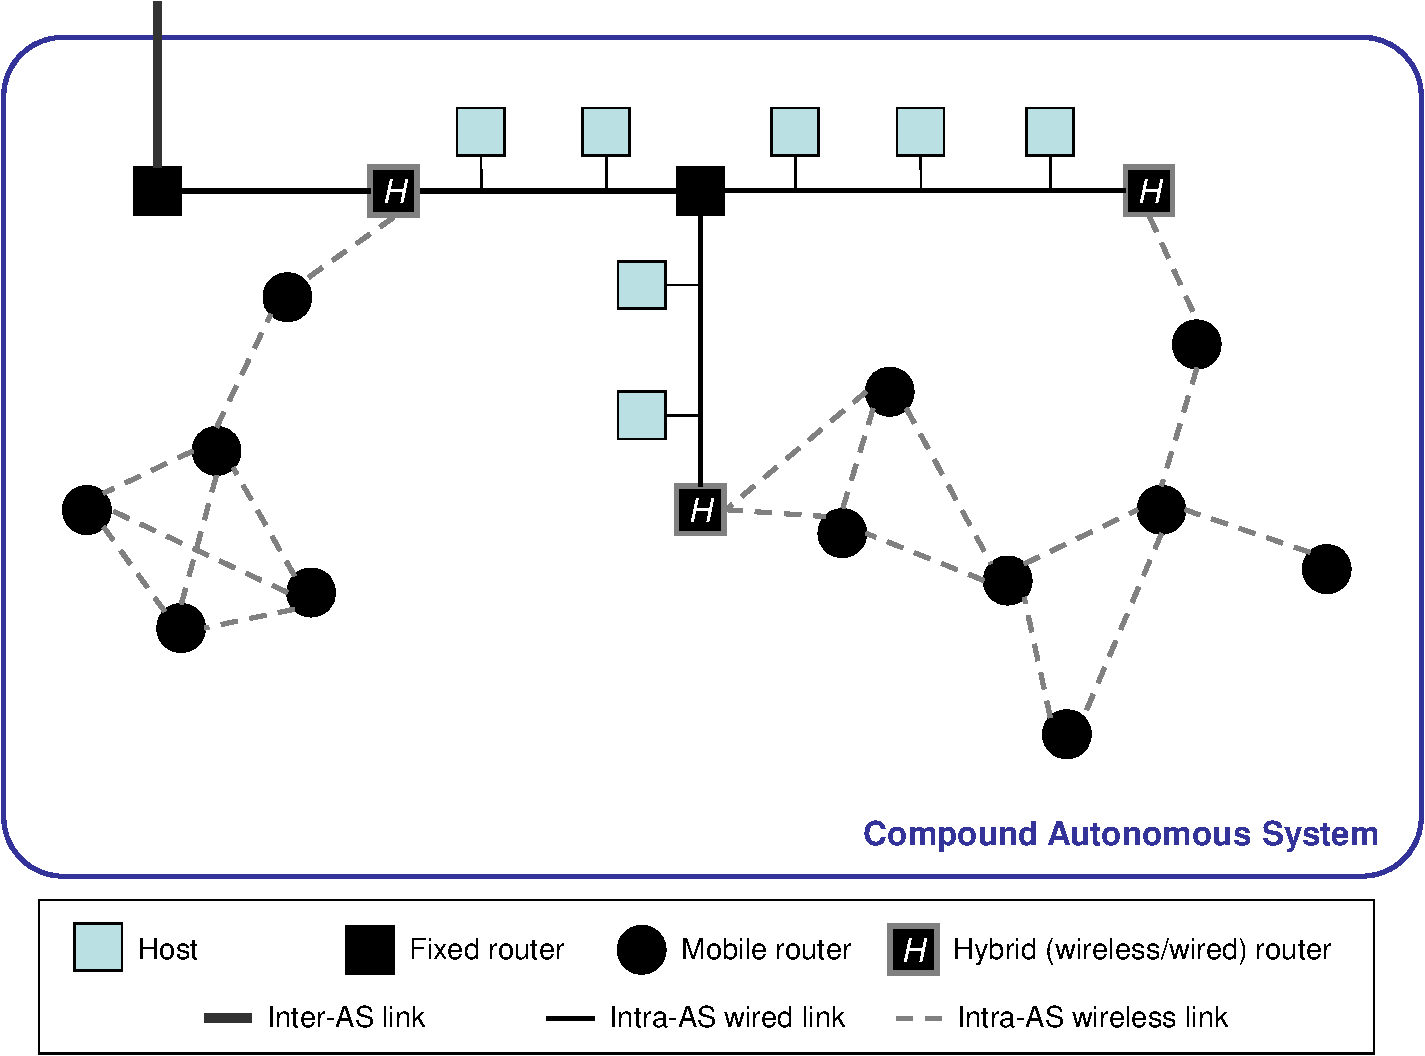
\includegraphics[width=0.8\textwidth]{Figures/cpd_as-crop.pdf}
\caption{A compound Autonomous System.}
\label{f:cpd_as}
\end{figure}
%
In these scenarios, a classic IGP (in IP networks, typically OSPF) is used for routing in the fixed network inside the AS. Rather than using an additional protocol for routing in the wireless mesh network inside the AS, it makes sense to explore approaches {\em extending} the protocol already used in the AS, so that it can take into consideration the issues described in section \ref{s:comm_wless}, run efficiently over wireless dynamic networks, handle the heterogeneity of the hybrid internetwork and thus perform routing over the whole compound AS. Extension for hybrid internetworks of a protocol already in use can significantly reduce the transition costs (technical implementation, engineer training...), as only minor changes, or no changes at all, will be needed in the networks using the original protocol. It may be also benefial in terms of networking management complexity and routing performance, as a single (extended) routing protocol is more bearable than several protocols running in different parts of the internetwork. In the latter case, route distribution between different protocols operating at wireless and wired networks needs to be performed in specific {\em hybrid routers} (see Figure \ref{f:cpd_as}); this adds another layer of networking complexity and is likely to cause routing suboptimality. The advantages of extending a protocol in use come, however, at the expense of increasing the complexity and narrowing the space for optimization in the extended protocol, which needs to cope efficiently with a broader range of networking scenarios.\ \\ \ \\
%
This section reviews the IETF extensions of the Open Shortest Path First (OSPF) protocol for MANETs. Section \ref{ss:ospf} shortly reviews the basics of OSPF, the main IGP for IP networks and a major representative of the link-state routing family, and indicates the reasons that prevent OSPF to be used ``as-is'' in wireless multi-hop ad hoc networks. Section \ref{ss:ospfmanet} describes the main elements of the three extensions for MANETs standardized by the IETF: Multi-Point Relays (MPR-OSPF, specified in RFC 5449), MANET Designated Routers (OSPF-MDR, specified in RFC 5614) and Overlapping Relays (OR/SP, specified in RFC 5820).
%
\subsection{Open Shortest Path First Protocol (OSPF)}
\label{ss:ospf}
%
OSPF \cite{rfc2328,rfc5340} is a link-state routing protocol for IP networks. Each router maintains a local {\bf Link State Database} (LSDB), representing the full network topology. The protocol ensures that each router has the same LSDB and, thus, the exact same view of the network topology. Paths to every possible destination are derived from the {\bf Shortest Path Tree} (SPT) that every router computes, by way of Dijkstra's algorithm \cite{dijkstra59}. \ \\ \ \\
%
Routers acquire information about their 2-hop (bi-directional) neighborhood and advertise their own presence and their 1-hop neighbors by periodically exchanging {\bf Hello} messages with all their neighbors, in the way described in section \ref{ss:nd}. \ \\ \ \\
%
Topology information is also disseminated through the network by way of {\bf Link State Advertisements} (LSAs). Each such LSA lists mainly the current adjacencies of the router which generated the LSA. The local LSDB stored by a router contains the most recent LSAs received from every other router in the network. \ \\ \ \\
%
Each router synchronizes its LSDB with a subset of its bidirectional neighbors. Synchronization between two neighboring routers is performed on a master-slave basis, by exchanging summaries of all LSAs in their LSDB, and then allowing each router to request retransmission of missing or locally outdated link-state advertisements. Links between a router and its synchronized neighbors are called {\bf adjacencies}. The set of adjancencies is expected to form a network-wide connected backbone, connecting all routers in the network, in order to ensure paths can be computed correctly.\ \\ \ \\
%
Finally, routers also acquire remote topology information by receiving LSAs. LSAs are flooded through the entire network in reliable fashion (explicit acknowledgements and retransmissions) via the backbone formed by adjacencies. Thus, any router which has formed adjacencies must advertise this periodically by way of constructing an LSA and performing LSA flooding.
%
\begin{equation}
\textrm{SPT links} \subset \textrm{Adjacent links} \subset \textrm{Bi-directional links}
\end{equation}
%
Remote topology information is then used for the construction of the Shortest Path Tree: each router computes the shortest paths based on the information contained in the set of received LSAs. \ \\ \ \\
%
This operation implies that OSPF exchanges control traffic and performs routing according to two principles:
%
\begin{enumerate}
\item Data traffic is routed to the corresponding destination through links contained in the Shortest Path Tree.
\item Data and control and traffic (LSAs and acknowledgements) is sent over adjacent (synchronized) links.
\end{enumerate}
%
\paragraph{Interface Types} 
%
Rules for flooding and adjacency handling vary for the different \emph{interface types} supported by OSPF. Four main interface types are specified in RFC 2328 \cite{rfc2328}:
%
\begin{itemize}
\item \emph{Point-to-point interfaces} are those connected to point-to-point links. Such a link only permits communicating with a single (neighboring) interface.
\item \emph{Broadcast interfaces} participate in a broadcast link, in which any interface can directly communicate with any other interface. A classic example of broadcast link is Ethernet.
\item \emph{Non-Broadcast Multiple Access (NBMA) interfaces}, for non-broadcast networks ({\em i.e.}, networks supporting more than two routers, but without broadcast capability) in which each pair of interfaces can communicate directly. This interface type may be used with X.25 and ATM networks with Switched Virtual Circuits (SVC).
\item \emph{Point-to-multipoint interfaces}, for those non-broadcast networks in which direct communication between any pair of interface is not guaranteed. This may be the case, for instance, in Frame Relay networks using only Permanent Virtual Circuits (PVC), if not every pair of routers have a PVC between them. 
\end{itemize}
%
OSPF only provides support for the two first interface types. In the NBMA and point-to-multipoint cases, OSPF {\em emulates} the behavior of a broadcast link and point-to-point links, repectively. For NBMA networks, LSA flooding and LSDB synchronization are handled by way of {\bf Designated Routers} (DRs). A Designated Router (as well as a Backup Designated Router, BDR, expected to become DR in case of DR's failure) is elected from among routers whose interfaces are connected to the same link. DRs (and BDRs) form adjacencies with all the routers connected to the same link, and the Designated Router becomes responsible for flooding of LSAs, originated by routers on that link. A router point-to-multipoint link, in turn, is handled as a set of independent point-to-point links, one per neighboring router with which direct communication is available.
%
\subsection{MANET Extensions: A Wireless Interface for OSPF}
\label{ss:ospfmanet}
%
Standard interface types for non-broadcast networks (point-to-multipoint and NBMA) are not adapted for operation in a wireless multi-hop ad hoc network. As discussed in section \ref{ss:issues}, routers in a wireless multi-hop network may not agree on which routers are connected to a given link. This implies that the DR-based mechanisms of NBMA cannot be directly used in wireless multi-hop ad hoc networks. DR election may be inconsistent between different routers, causing flooding to disfunction and, possibly even preventing the protocol from converging. The use of the point-to-point interface, in turn, does not scale in these dynamic networks: point-to-point emulation for every pair of interfaces directly reachable to each other causes an excessive control traffic overhead, even for relatively small networks, as shown experimentally in Henderson {\em et al.} \cite{henderson03}. This fact has led the research and industrial OSPF community to develop a new interface type to support the characteristics of wireless multi-hop ad hoc networks.\ \\ \ \\
%
This new interface type needs to optimize the operation of (1) describing local topology in LSAs, (2) performing LSA flooding and (3) establishing and maintaining adjacencies in the context of wireless communication. Different approaches have been explored at the IETF, which have led to three different extensions of OSPF, consisting of three different interfaces for wireless multi-hop networks (or MANETs, in IETF's terminology).
%
\paragraph{Multi-Point Relays} MPR-OSPF \cite{rfc5449} use Multi-Point Relays (MPR \cite{mpr-hicss2002}, see section \ref{ss:flood}) to optimize topology description, LSA flooding and LSDB synchronization. Nodes select MPRs from among their bidirectional neighbors in order to provide 2-hop coverage, and use them to disseminate their LSAs. A router becomes adjacent to both neighbors which it has selected as multi-point relays (MPRs) and neighbors which have selected the router as their multi-point relay (MPR selectors). Each router advertises in its LSAs its own MPRs and MPR selectors; consequently, the Shortest Path Tree is constructed over the set of adjacencies. 
%
\paragraph{Overlapping Relays \& Smart Peering} The Overlapping Relays / Smart Peering (OR/SP) extension of OSPF \cite{rfc5820} floods LSAs via MPR as in MPR-OSPF, where the multi-point relays selected among the adjacent (synchronized) neighbors of the electing router. Adjacencies are selected following the Smart Peering (SP) rule, in which a neighbor becomes adjacent if it is not already reachable through the computing router's current Shortest Path Tree. The SP criterion reduces dramatically the number of synchronized links in the network. LSAs list adjacent neighbors, and may also list additional bidirectional neighbors (so-called \emph{unsynchronized adjacencies}). The SPT is thus constructed over adjacencies and a subset of bidirectional neighbors. 
%
\paragraph{MANET Designated Routers} OSPF-MDR \cite{rfc5614} relies on two Connected Dominating Sets (CDS): the MANET Designated Routers (MDR) backbone and the Backup MDRs (BMDR) backbone. Both extend the standard OSPF (for NBMA networks) notions of ``Designated Routers" and ``Backup Designated Routers" to MANETs. This implies that routers behave differently depending on their role. MDRs are the only nodes allowed to flood LSAs. Every non-MDR router becomes adjacent at least to the closest MDR, and MDRs must become adjacent to other MDRs. LSAs list a configurable subset of links of the originator, which must at least include the adjacent neighbors. The SPT is thus constructed over adjacencies and a subset of bidirectional neighbors. \ \\ \ \\
%
Compatibility with the OSPF routing philosophy detailed in section \ref{ss:ospf} varies significantly depending on the considered OSPF extension. MPR-OSPF is designed to preserve the two principles in OSPF routing: shortest, synchronized paths for data traffic and synchronized links for control traffic. Under the Overlapping Relays extension, data traffic paths are synchronized, but they are not necessarily optimal, as routers only synchronize a small fraction of their available links. Although providing several configuration parameters to tune the protocol's performance, the MANET Designated Routers (OSPF-MDR) also try to minimize the control traffic by reducing the number of synchronized links, even when this may lead to path suboptimality for data traffic.
%
\paragraph{Preserving OSPF routing principles} Performed experiments suggest that extensions providing (theoretical) shortest paths for data traffic achieve a better performance than those neglecting shortest paths or allowing suboptimal routing in a wireless multi-hop network \cite{aircc, porto}. Further analysis showed that preserving the second principle (all traffic is sent over synchronized links) in OSPF over mobile ad hoc networks, in the way that MPR-OSPF does, requires a significant amount of overhead due to the LSDB exchange between routers becoming {\em adjacent} (synchronized), and does not bring substantial benefit, due to short lifetime of several synchronized links in a wireless multi-hop dynamic network \cite{hicss2011}.
%
\paragraph{Why maintain LSDB synchronization in Extended OSPF ?} LSDB synchronization between two routers proves useful in classic (wired) Internet internetworks, but is an expensive operation to perform in a dynamic (wireless multi-hop or mobile ad hoc) network. This is the reason why other link-state protocols such as OLSR, designed specifically for wireless mesh and mobile ad hoc networks, does not provide any mechanism for synchronizing the LSDBs of neighboring routers: topology information is only disseminated through the network by way of LSA flooding (see section \ref{sec:olsr}). In the case of extended OSPF, there are two reasons for maintaining the notion of LSDB synchronization: 
%
\begin{enumerate}
\item {\bf OSPF backwards compatibility}. In standard OSPF \cite{rfc2328,rfc5340}, the notion of {\em adjacency} is essential in the protocol's architecture and the router's operation, regardless of the specific types used for running OSPF in the router's interfaces.
\item {\bf Routing in heterogeneous internetworks}. Unlike OLSR, extended OSPF is expected to run over hybrid internetworks (or compound Autonomous Systems, see Figure \ref{f:cpd_as}), that is, internetworks in which wired networks handled by standard OSPF interface types coexist and are interconnected with wireless multi-hop networks using the adapted wireless interface of (extended) OSPF. In these scenarios, in which some nodes (with wireless interfaces) are exposed to frequent disconnections from the network (meaning that their LSDBs may be no longer updated for a while) and others maintain stable links with their neighbors (those with wired interfaces), the fact that every router is expected to synchronize its LSDB with {\em at least} one of its neighbors provides an upper bound for the maximum time that a router $A$ (in the wireless region of the internetwork) stays {\em disconnected} (that is, unaware of its local topology) from another router $B$ (in the wired region of the internetwork) after missing an LSA flooded by router $B$. This becomes an issue as the time between consecutive LSA flooding processes from $B$ is typically high -- as wired links are stable and thus require less frequent updates about their state than wireless ones.
\end{enumerate}
%
\paragraph{Further Extensions: adapted LSDB synchronization, MPR+SP and SLOT-OSPF} In this context, some additional approaches can be explored beyond the three standardized extensions of OSPF. Clausen {\em et al.} \cite{secon2004}, for example, propose a LSDB synchronization process based on the periodic broadcasting of {\em signatures} of the LSDB by every router to its neighborhood. These signatures allow neighbors of the originator to detect topology inconsistencies with its own LSDB, and request unicast retransmission of the corresponding LSAs. This turns the standard OSPF synchronization mechanism, based on a router-to-router LSDB exchange, to a router-to-neighborhood mechanism that takes advantage from the semibroadcast nature of communication in a wireless multi-hop network.

Without modifying the standard OSPF adjacency-forming process, LSDB synchronization can be kept, but the number of adjacencies per router should be reduced as much as possible, given the high cost of synchronization in terms of overhead and its small benefit in a dynamic network, with short-lived links. Data traffic should be sent over shortest paths (that is, optimal paths over the network, according to the available LSDB information and the metric in use), but these paths do not need to be synchronized. This leads to combine in the same OSPF extension the mechanisms to provide shortest paths (MPR selection for topology description) and the mechanisms reducing the most the number of adjacencies to be established per router ({\em e.g.}, the Smart Peering rule used in the Overlapping Relays extension). The resulting extension, denominated MPR+SP, presents a better routing performance than extensions MPR-OSPF and OR/SP in which it is based, as shown in Cordero {\em et al.} \cite{hicss2011}. Similarly, extension SLOT-OSPF \cite{mass2010} using the Relative Neighbor Graph (RNG \cite{toussaint80}) for establishing adjacencies and MPR selection for computing shortest paths, also achieves better results in terms of delivery ratio and control traffic overhead than the standard extension to which it compares. In both cases (MPR+SP and SLOT-OSPF) shortest path computation, for which a comprehensive view of the network topology (with most of the links) is required, is splitted from the adjacency-forming criterion, which aims to reduce as much as possible the number of LSDB synchronizations to be performed. This split enables a further optimization of the protocol routing performance.




%This appendix contains a few exercises on the evolution of transport protocols and their interactions with middleboxes.

\subsection{Transport protocols}

\begin{enumerate}

\item TCP provides a reliable transport service. Assuming that you control the two endpoints of a connection, how would you modify the TCP protocol to provide an unreliable service ? Explore two variants of such a transport service :
  \begin{itemize}
  \item an unreliable bytestream where bytes can be corrupted but where there are no losses
  \item an unreliable bytestream that prevents data corruption but can deliver holes in the bytestream
  \end{itemize}

\item Same question as above, but for SCTP.

\item TCP provides a connection-oriented bytestream service. How would you modify TCP to support a message-oriented service. Consider two variants of this service :
 \begin{itemize}
    \item A connection-oriented message-mode service that supports only small messages, i.e. all messages are smaller than one segment.
    \item A connection-oriented message-mode service that supports any message length. 
 \end{itemize}

\item The large windows extension for TCP defined in \cite{rfc1323} uses the \texttt{WScale} option to negotiate a scaling factor which is valid for the entire duration of the connection. Propose another method to transport a larger window by using a new type of option inside each segment. What are the advantages/drawbacks of this approach compared to \cite{rfc1323} assuming that there are no middleboxes ?

\item One of the issues that limits the extensibility of TCP is the limited amount of space to encode TCP options. This limited space is particularly penalizing in the SYN segment. Explore two possible ways of reducing the consumption of precious TCP option-space
\begin{itemize}
\item Define a new option that packs several related options in a smaller option. For example try to combine SACK with Timestamp and Window scale in a small option for the SYN segment. 
\item Define a compression scheme that allows to pack TCP options in fewer bytes. The utilisation of this compression scheme would of course need to be negotiated during the three way handshake.
\end{itemize}



\end{enumerate}

\subsection{Middleboxes}

Middleboxes may perform various changes and checks on the packets that they process.  Testing  real middleboxes can be difficult because it involves installing complex and sometimes costly devices. However, getting an understanding of the interactions between middleboxes and transport protocols can be useful for protocol designers. 

A first approach to understand the impact of middleboxes on transport protocols is to emulate the interference caused by middleboxes.This can be performed by using \texttt{click} \cite{Kohler_click:2000} elements that emulate the operation of middleboxes \cite{Hesmans_click:2013} : 
\begin{itemize}
\item \texttt{ChangeSeqElement} changes the sequence number in the TCP header of processed segments to model a firewall that randomises sequence numbers
\item \texttt{RemoveTCPOptionElement} selectively removes a chosen option from processed TCP segments
\item \texttt{SegSplitElement} selectively splits a TCP segment in two different segments and copies the options in one or both segments
\item \texttt{SegCoalElement} selectively coalesces consecutive segments and uses the TCP option from the first/second segment for the coalesced one
\end{itemize}

Using some of these \texttt{click} elements, perform the following tests with one TCP implementation. 

\begin{enumerate}

\item Using a TCP implementation that supports the timestamp option defined in \cite{rfc1323} evaluate the effect of removing this option in the \texttt{SYN}, \texttt{SYN+ACK} or regular TCP segments with the \texttt{RemoveTCPOptionElement} \texttt{click} element.

\item Using a TCP implementation that supports the selective acknowledgement option defined in \cite{rfc2018} predict the effect randomizing the sequence number in the TCP header without updating anything in this option as done by some firewalls. Use the \texttt{ChangeSeqElement} \texttt{click} element to experimentally verify your answer. Instead of using random sequence numbers, evaluate the impact of logarithmically increasing/decreasing the sequence numbers (i.e. +10, +100, +1000, +1000, \ldots)

\item Recent TCP implementations support the large windows extension defined in \cite{rfc1323}. This extension uses the \texttt{WScale} option in the \texttt{SYN} and \texttt{SYN+ACK} segments. Evaluate the impact of removing this option in one of these segments with the \texttt{RemoveTCPOptionElement} element. For the experiments, try to force the utilisation of a large receive window by configuring your TCP stack.

\item Some middleboxes split or coalesce segments. Considering Multipath TCP, discuss the impact of splitting and coalescing segments on the correct operation of the protocol. Use the Multipath TCP implementation in the Linux kernel and the \texttt{SegCoalElement} and \texttt{SegSplitElement} \texttt{click} elements to experimentally verify your answer.

%\item Using the Multipath TCP implementation in the Linux kernel and one of the above mentioned \texttt{click} elements, 


\item The extensibility of SCTP depends on the utilisation of chunks. Consider an SCTP-aware middlebox that recognizes the standard SCTP chunks but drops the new ones. Consider for example the partial-reliability extension defined in \cite{rfc3758}. Develop a \texttt{click} element that allows to selectively remove a chunk from processed segments and evaluate experimentally its impact on SCTP.

\end{enumerate}

Another way to evaluate middleboxes is to try to infer their presence in a network by sending probe packets. This is the approach used by Michio Honda and his colleagues in \cite{honda2011still}. However, the TCPExposure software requires the utilisation of a special server and thus only allows to probe the path towards this particular server. An alternative is to use \texttt{tracebox} \cite{Detal_Tracebox:2013}. \texttt{tracebox} is an extension to the popular \texttt{traceroute} tool that allows to detect middleboxes on (almost) any path. \texttt{tracebox} sends TCP and UDP segments inside IP packets that have different Time-To-Live values like \texttt{traceroute}. When an IPv4 router receives an IPv4 packet whose TTL is going to expire, it returns an ICMPv4 \emph{Time Exceeded} packet that contains the offending packet. Older routers return in the ICMP the IP header of the original packet and the first 64 bits of the payload of this packet. When the packet contains a TCP segment, these first 64 bits correspond to the source and destination ports and the sequence number. However, recent measurements show that a large fraction of IP routers in the Internet, notably in the core, comply with \cite{rfc1812} and thus return the complete original packet. \texttt{tracebox} compares the packet returned inside the ICMP message with the original one to detect any modification performed by middleboxes. All the packets sent and received by \texttt{tracebox} are recorded as a libpcap file that can be easily processed by using \texttt{tcpdump} or \texttt{wireshark}.


\begin{enumerate}

\item Use \texttt{tracebox} to detect whether the TCP sequence numbers of the segments that your host sends are modified by intermediate firewalls or proxies.

\item Use \texttt{tracebox} behind a Network Address Translator to see whether \texttt{tracebox} is able to detect the modifications performed by the NAT. Try with TCP, UDP and regular IP packets to see whether the results vary with the protocol. Analyse the collected packet traces.

\item Some firewalls and middleboxes change the \texttt{MSS} option in the \texttt{SYN} segments that they process. Can you explain a possible reason for this change ? Use \texttt{tracebox} to verify whether there is a middlebox that performs this change inside your network.

\item Use \texttt{tracebox} to detect whether the middleboxes that are deployed in your network allow new TCP options, such as the ones used by Multipath TCP, to pass through.

\item Extend \texttt{tracebox} so that it supports the transmission of SCTP segments containing various types of chunks.


\end{enumerate}


\subsection{Multipath TCP}

Although Multipath TCP is a relatively young extension to TCP, it is already possible to perform interesting experiments and simulations with it. The following resources can be useful to experiment with Multipath TCP :

\begin{itemize}
\item \url{http://www.multipath-tcp.org} provides an implementation of Multipath TCP in the Linux kernel with complete source code and binary packages. This implementation covers most of \cite{rfc6824} and supports the coupled congestion control \cite{rfc6356} and OLIA \cite{olia}. Mininet and netkit images containing the Multipath TCP kernel are available from the above website.
\item \url{http://caia.swin.edu.au/urp/newtcp/mptcp/} provides a kernel patch that enables Multipath TCP in the FreeBSD-10.x kernel. This implementation only supports a subset of \cite{rfc6824}
\item The \texttt{ns-3} network simulator\footnote{See \url{http://www.nsnam.org/}.} contains two forms of support for Multipath TCP. The first one is by using a Multipath TCP model\footnote{See \url{https://code.google.com/p/mptcp-ns3/}}. The second is by executing a modified Linux kernel inside \texttt{ns-3}  by using Direct Code Execution\footnote{See \url{http://www.nsnam.org/projects/direct-code-execution/}}.

\end{itemize}

Most of the exercises below can be performed by using one of the above mentioned simulators or implementation. 

\begin{enumerate}

\item Several congestion control schemes have been proposed for Multipath TCP and some of them have been implemented. Compare the performance of the congestion control algorithms that your implementation supports. 

\item The Multipath TCP congestion control scheme was designed to move traffic away from congested paths. TCP detects congestion through losses. Devise an experiment using one of the above mentioned simulators/implementation to analyse the performance of Multipath TCP when losses occur.

\item The non-standard \texttt{TCP\_INFO} socket option\cite{Pfeiffer_Measuring:2007} in the Linux kernel allows to collect information about any active TCP connection. Develop an application that uses \texttt{TCP\_INFO} to study the evolution of the Multipath TCP congestion windows.


\item Using the Multipath TCP  Mininet or netkit image, experiment with Multipath TCP's fallback mechanism by using \texttt{ftp} to transfer files through a NAT that includes an application level gateway. Collect the packet trace and verify that the fallback works correctly.

\end{enumerate}



%\subsection {Minion}


%\ed{Any suggestion from Jana ?} 


%\ed{A one page conclusion.} 
%Something on evolution of transport
%Something on Middleboxes
%Something on MPTCP
%Something on Minion
%One paragraph on the future

The Transport Layer in the Internet evolved for nearly two decades,
but it has been stuck for over a decade now.
A proliferation of middleboxes in the Internet,
devices in the network that look past the IP header,
has shifted the waist of the Internet hourglass 
upward from IP
to include UDP and TCP,
the legacy workhorses of the Internet.
While popular for many
different reasons, 
middleboxes thus deviate from the Internet’s
end-to-end design, creating large deployment
“black-holes”---singularities where legacy transports get through, but
any new transport technology or protocol fails,
severely limiting transport protocol evolution.
The fallout of this ossification
is that new transport protocols,
such as SCTP and DCCP,
that were developed to offer much needed 
richer end-to-end services to applications,
have had trouble getting deployed since they require changes 
to extant middleboxes.

Multipath TCP is perhaps the most significant change to TCP in the past twenty
years. It allows existing TCP applications to achieve better
performance and robustness over today's networks, and it has been
standardized at the IETF. The Linux kernel implementation shows that
these benefits can be obtained in practice.  However, as with any
change to TCP, the deployment bar for Multipath TCP is very high: only
time will tell whether the benefits it brings will outweigh the added
complexity it brings in the end-host stacks.

The design of Multipath TCP has been a lengthy, painful process that took around five
years. Most of the difficulty came from the need to support existing middlebox
behaviors, while offering the exact same service to applications as TCP. Although
the design space seemed wide open in the beginning, in the end we were \emph{just} able
to evolve TCP this way: for many of the design choices there was only one viable option
that could be used. When the next major TCP extension is designed in a network with even more
middleboxes, will we, as a community, be as lucky?

A pragmatic answer to the inability to deploy new transport protocols
is Minion. It allows deploying new transport services 
by being backward compatible with middleboxes by encapsulating new protocols inside TCP.
Minion demonstrates that it is possible to obtain
unordered delivery and multistreaming
from wire-compatible TCP and TLS streams
with surprisingly small changes to TCP stacks
and application-level code.
Minion offers a path toward
the performance benefits of unordered delivery,
which we expect to be useful to applications
that use TCP for a variety of pragmatic reasons.

%Minion is just the latest in an ever-growing encapsulation war that 
%has engulfed end-hosts and network providers for years on end. 
Early in the Internet's history,
all IP packets could travel freely through the Internet, as IP was the narrow waist of
the protocol stack. 
Eventually, 
apps started using UDP and TCP exclusively,
and some, such as Skype, used them adaptively,
probably due to security concerns
in addition to the increasing proliferation of middleboxes that allowed only UDP and TCP through.
As a result, UDP and TCP over IP were then perceived to constitute the new waist of the Internet.
(We'll note that HTTP has also recently
been suggested as the new waist~\cite{popa10http}.) 
%UDP is not that great getting through newer firewalls either, so TCP is the new narrow
%waist, or even HTTP as recently proposed. 

Our observation is that
whatever the new waist is,
middleboxes will embrace it and optimize for it: 
if MPTCP and/or Minion become popular, 
it is likely that middleboxes will be devised that understand these protocols
to optimize for the most successful use-case of these protocols
and to help protect any vulnerable applications using them.
One immediate answer from an application would be to
use the encrypted communication proposed in Minion---%
but actively hiding information from a network operator
can potentially encourage the network operator
to embed middleboxes that intercept encrypted connections,
effectively mounting man-in-the-middle attacks
to control traffic over their network,
as is already being done in several corporate firewalls~\cite{marko10using}.
%a potential serious security breach, and many ISPs
%may either drop traffic or require their customers to ``install'' keys in the 
%browser that effectively allow middleboxes to become a man-in-the-middle of the TLS connection. 
To bypass these middleboxes,
new applications may encapsulate their data {\em even} deeper,
leading to a vicious circle resembling an ``arms race'' for control
over network use.
% them looking even deeper in the packets. As we can see, 
%this is a vicious circle that no-one can ever win.

This ``arms race'' is a symptom of a fundamental tussle between
end-hosts and the network: end-hosts will always want to deploy new
applications and services, while the network will always want to allow and optimize only
existing ones~\cite{tussle}.
To break out of this vicious circle,
we propose that
end-hosts and the network must co-operate,
and that they must build cooperation into their protocols.
Designing and providing protocols and incentives for this cooperation may hold the key to creating a
truly evolvable transport (and Internet) architecture.


%\newpage

\addcontentsline{toc}{section}{References}

%\bibliographystyle{ieeetr}
% Define style for bibtex bibliography
\bibliographystyle{../acm}
\bibliography{rfc,bibliography}

%\newpage

\addcontentsline{toc}{section}{Glossary}
\glsaddall
\printglossaries

% that's all folks
\end{document}


